%=======================================================================
%  Transformer-based, topology-preserving, temporally consistent segmentation
%  and tracking of individual neurons in phase-contrast time-lapse microscopy
%
%  Target: Cell Reports Methods
%  Structure: 1 Intro · 2 Related Work · 3 Methods · 4 Results · 5 Discussion
%
%  HOW TO USE IN OVERLEAF
%   1. Paste this file as main.tex
%   2. Upload refs.bib to the project ROOT
%   3. Create a folder "figures/" and upload the figures into it
%      (charts are vector .pdf; photographic panels are .png)
%   4. Compile with pdfLaTeX  (Figures 1, 2 and 3 are native TikZ - no PNG needed)
%
%  CURRENT LAYOUT -- 9 figures / 3 tables:
%    Fig 1 pipeline (Intro, TikZ)      Fig 2 architecture (3.2, TikZ)
%    Fig 3 whytopology (3.4, TikZ)     Fig 4 benchmark (4.1)
%    Fig 5 temporal (4.2)              Fig 6 qualitative (4.3)
%    Fig 7 culture / Fig 8 proofA81 / Fig 9 rawoutput  (all appendix)
%    Tab 1 main (4.1)   Tab 2 drift (4.2)   Tab 3 protocol (appendix)
%  The loss-terms table was removed 2026-09: Eq. 3 already gives the four
%  weights and the surrounding prose gives each term's rationale, so it
%  restated the section rather than adding to it.
%  Fig 3 was Fig 6 until it moved from Ablations into 3.4, where it is first
%  cited -- placeins[section] will not let a float cross a \section boundary.
%  KEEP EVERY FLOAT DECLARED IMMEDIATELY AFTER THE PARAGRAPH THAT FIRST CITES IT;
%  parking them at the end of a subsection is what made them bunch up before.
%=======================================================================
\documentclass[11pt,a4paper]{article}
%------------------------- packages ----------------------------------
\usepackage[utf8]{inputenc}
\usepackage[T1]{fontenc}
\usepackage{lmodern}
\usepackage[margin=2.4cm]{geometry}
\usepackage{graphicx}
\usepackage{booktabs}
\usepackage{array}
% left-aligned wrapping column, so p{} cells do not stretch their spaces
\newcolumntype{L}[1]{>{\raggedright\arraybackslash}p{#1}}
\usepackage{amsmath,amssymb}
\usepackage{siunitx}
\usepackage{xcolor}
\usepackage[labelfont=bf,font=small]{caption}
\usepackage{authblk}
\usepackage{lineno}
\usepackage[section]{placeins}   % keeps floats from crossing \section boundaries
% placeins[section] does NOT barrier at \subsection, so within a section every
% float can drift across subsection boundaries and they bunch up at the end.
% Add the same barrier at \subsection (starred form included).
\makeatletter
\let\SD@subsection\subsection
\renewcommand\subsection{\FloatBarrier\@ifstar{\SD@subsection*}{\SD@subsection}}
\makeatother
% LaTeX's defaults reserve most of a page for text (textfraction 0.2) and allow
% only two floats at the top, so with a barrier at each subsection the floats
% that cannot be placed pile up at the barrier. Loosening the fractions lets
% them sit on the same pages as the text that discusses them.
\renewcommand{\topfraction}{0.9}
\renewcommand{\bottomfraction}{0.7}
\renewcommand{\textfraction}{0.1}
\renewcommand{\floatpagefraction}{0.75}
\setcounter{topnumber}{3}
\setcounter{bottomnumber}{2}
\setcounter{totalnumber}{4}
\usepackage{tikz}
\usetikzlibrary{arrows.meta,positioning,calc,backgrounds,decorations.pathreplacing,shapes.arrows}
\usepackage[numbers,sort&compress]{natbib}
\PassOptionsToPackage{hyphens}{url}
\usepackage[colorlinks=true,allcolors=blue!60!black]{hyperref}

\graphicspath{{figures/}}

%--- FAST-COMPILE SWITCH ----------------------------------------------------
% Uncomment ONE line below to replace every image with an outlined box. This
% cuts compile time to a few seconds when you are only editing prose.
%
% This is safe here in a way a bare \usepackage[draft]{graphicx} is NOT. In
% draft mode LaTeX never opens the image files, so it cannot know their shape;
% a figure given only a width is then drawn as a SQUARE, which is what emptied
% whole pages in earlier drafts. Every \includegraphics in this file therefore
% carries an explicit height as well as a width (plus keepaspectratio, so the
% real build still scales to fit and cannot distort anything). The draft boxes
% consequently have the true aspect ratio and floats land exactly where they
% land in a full build.
%
% COMMENT IT OUT AGAIN BEFORE SUBMITTING -- the boxes are not the figures.
\setkeys{Gin}{draft}   % <-- ON: images are boxes. Comment out for the real build.
%----------------------------------------------------------------------------
%\linenumbers                  % uncomment for review (slows compiles)
\setlength{\parskip}{0.35em}

% A float at the top of a page can strand the last line of the paragraph that
% preceded it -- one orphan line under Table 3, which is what "tionately severe
% penalty during these early frames." was. LaTeX's defaults (150) barely
% discourage this; 10000 forbids it, so the break moves up and takes at least
% two lines with it. displaywidowpenalty covers the same case around equations.
\widowpenalty=10000
\clubpenalty=10000
\displaywidowpenalty=10000

\newcommand{\todo}[1]{\textcolor{red!80!black}{\textbf{[TODO: #1]}}}
\newcommand{\note}[1]{\textcolor{blue!60!black}{\textit{(#1)}}}

% ---- figure palette (matches the PNG figures) ----
\definecolor{navy}{HTML}{16324F}
\definecolor{ourblue}{HTML}{1F6FB2}
\definecolor{teal}{HTML}{2CA6A4}
\definecolor{softgrey}{HTML}{E4E8ED}
\definecolor{midgrey}{HTML}{8B96A3}
\definecolor{amber}{HTML}{E1A93B}
\definecolor{crimson}{HTML}{C0392B}

%------------------------- title -------------------------------------
\title{\textbf{NeuroVestigo: topology-preserving segmentation and tracking
of single neurons in phase-contrast time-lapse microscopy}}

% Author order to be confirmed with Prof. Shefi.
% E. N. Berkovich acquired and hand-annotated the time-lapse dataset
% (M.Sc. thesis, BIU 2025) - see \cite{berkovich2025neurite}.
\author[1]{Adi Oizerovich}
\author[1]{Efrat Naomi Berkovich}
\author[1]{Sharon Cohen}
\author[1]{Ofek Ophir}
\author[1,*]{Orit Shefi}
\affil[1]{Faculty of Engineering, Bar-Ilan University, Ramat Gan, Israel}
\affil[*]{Correspondence: adi.oizerovich@gmail.com}
\date{}

%=====================================================================
%  NUMBERS TO REFRESH AFTER THE FINAL TRAINING RUN
%  ------------------------------------------------------------------
%  CHECKPOINT DIRECTORIES (2026-09). Only two exist and both are live:
%    checkpoints/            SHIPPED -- 22 training recordings
%    checkpoints-16-frames/  PREVIOUS -- 20 training recordings
%  gpu-checkpoints/ has been DELETED. It was the superseded 8-frame /
%  topology_resolution 256 run, and it is where the "8-frame validation"
%  label on Figure 4 came from. Do not reinstate it.
%
%  SHIPPED MODEL: checkpoints/lora_weights.pt -- focal 3 / Dice 2 /
%  cbDice 0.3 / supervoxel 0.3, topology_resolution 512, clips of 16 frames,
%  22 training recordings. 110 epochs; BEST CHECKPOINT epoch 90.
%  TEST (t>=1, full propagation): IoU 0.763 Dice 0.864 cbDice 0.855 clDice 0.946
%  Validation is 0.8399 IoU at epoch 90 -- kept OUT of the paper deliberately.
%  DL convention reports the test set; validation is what the model was
%  selected on, so reporting it as a result is circular. It appears only
%  where it justifies a competitor setting (Appendix).
%
%  PROTOCOL FACTS verified against checkpoints/training_config.json (2026-09):
%    num_frames 16, val_num_frames 16 -> VALIDATION CLIPS ARE ALSO 16 FRAMES
%    clip_stride 4, batch 2, 110 epochs, seed 42, hiera_rank 8
%    early_stopping_patience 90 -> NEVER TRIGGERED; ran the full budget
%    3.12 s/step (from the log); ~17 h total
%  CAVEAT: the run RESUMED, and training_log.json now holds only epochs
%  108-110, so best-epoch 90 / val_iou 0.8399 and the total wall-clock are
%  NOT verifiable from the repo -- they come from Adi. Steps/epoch is derived
%  (177); the same derivation gives 157 for the previous run, whose recorded
%  value was 156, so treat the hours figure as approximate.
%
%  PREVIOUS MODEL (checkpoints-16-frames, 20 recordings, best epoch 100):
%    TEST IoU 0.760 Dice 0.861 cbDice 0.851 clDice 0.943, val_iou 0.8377
%  Adding the two recordings moved test IoU by +0.003 and left the decay at
%  0.070. Written up as the "Training-set size" ablation; the larger set is
%  shipped because it is the one released, not because it scores better.
%
%  WHY THIS RUN (bake-off of five, all scored identically, Aug 2026):
%    D      3/2/0.3/0.3, topo_res 256 (BUGGY loss)  -- test cbDice 0.847
%    fixed  3/2/0.3/0.3, topo_res 512               -- test cbDice 0.849
%    F      5/2/1.0/0.3, topo_res 512               -- test cbDice 0.843
%    16-fr  3/2/0.3/0.3, topo_res 512, 16-frame clips -- test cbDice 0.851 <- SHIPPED
%  D, fixed and F are statistically indistinguishable (paired over 9 recordings,
%  p=0.26..1.00) and their VALIDATION ranking is the exact REVERSE of their TEST
%  ranking -- the signature of noise. cbDice weight 0.3 -> 1.0 changes nothing
%  measurable even with the loss corrected. Do not re-run loss-weight sweeps.
%  The 16-frame run is the only one that wins the mean on all four metrics on
%  BOTH splits (8/8 comparisons in the same direction); clDice, the metric NOT
%  in the loss, wins 7/9 recordings (Wilcoxon p=0.039 -- would not survive
%  Bonferroni across four metrics, so treat as suggestive).
%
%  DRIFT (cbDice by quartile of each test recording) -- the real deficit, and
%  ~25x larger than any loss-weight effect. Decay is Q4-Q1 (full span). An
%  earlier draft used Q4-Q2, which is arbitrary AND changes a ranking: under
%  Q4-Q2 Cellpose -0.160 vs SAM 2 -0.166, under Q4-Q1 -0.130 vs -0.207. Q1 is
%  the honest baseline; SAM 2 simply drops hardest right after its prompt
%  (Q1 0.844 -> Q2 0.802), which Q4-Q2 hides. Do not revert.
%    run      Q1     Q2     Q3     Q4    Q4-Q1
%    fixed  0.878  0.889  0.835  0.794  -0.084
%    16-fr  0.876  0.887  0.833  0.807  -0.069
%  RECOMPUTED 2026-08-27 by benchmark/drift_quartiles.py, which is now the ONLY
%  source for Table 3 -- all seven rows come from one run of it. The previous
%  numbers were ~0.005 lower across the board and could not be reproduced by any
%  quartile convention or predictions directory; do not mix the two.
%  SAM 3.1 decays -0.418, 6.1x ours, despite 10 GT points on EVERY frame.
%  The 16-frame gain is entirely in Q4 (0.785 -> 0.799) with Q1-Q3 unchanged --
%  exactly what doubling the backprop-through-time horizon should produce.
%
%  RESOLVED: the rank-16 encoder run (Hiera blocks 10-11, up from rank 8)
%  OVERFITTED and was rejected. Rank 8 stands, and with it the 13.9%% /
%  5,557,250 / 914,432 parameter figures throughout. This VALIDATES the
%  argument Sec. 3.2 already makes on principle -- that adapting the encoder
%  harder on 25 recordings degrades rather than specialises it. The checkpoint
%  was not copied off the cluster, so Sec. 4.3 carries no numbers for it; if
%  the validation curve can be recovered it becomes a fourth ablation and turns
%  that paragraph from asserted into measured.
%
%  VENUE: ISBI 2027. Finish the full-length paper first, then compress. ISBI is
%  ~4 pages incl. figures, so expect to drop Eq. 4-8, the competitor-protocol
%  appendix and most of Sec. 3.3; keep Table 2 (benchmark), Table 3 (drift) and
%  one qualitative figure.
%
%  COMPETITOR FAIRNESS, third pass (2026-08-11): Cellpose-SAM's flow_threshold
%  was never swept -- sweep_cellpose.py advertised it in the docstring but the
%  grid was scale x cellprob x invert only. cellpose DISCARDS masks whose flow
%  error exceeds it, and thin neurites produce atypical flow fields, so the
%  default 0.4 was binning valid detections: 0 instances on 37/72 frames of
%  A71_C1. Swept on validation (benchmark/sweep_cellpose_flow.py): IoU .440 at
%  0.4 rising to a .564 plateau from 1.0 up, empty frames 3/40 -> 0/40; 1.5
%  selected, applied unchanged to test. TEST effect: IoU .295 -> .563,
%  cbDice .339 -> .683. Checked for reassembly artefact: the union-matching
%  protocol merges 11.5 instances/frame into Cellpose's target vs 24.9 for
%  Omnipose, so Cellpose is NOT specially favoured -- it was uniquely
%  handicapped. normalize=False scores higher still but only by shattering the
%  frame into ~4900 instances; excluded as a scoring artefact.
%
%  uSAM MASK-SELECTION AUDIT (2026-08-18), prompted by the red blow-ups Adi
%  spotted in single_frame_compare. NOT our bug. uSAM returns 3 candidate masks
%  and we keep its own top-scoring one (documented usage). On 29/328 test frames
%  (9%%), none earlier than 71%% through a recording (median 89%%), it returns a
%  mask >3x the GT area AND ranks it above a better mask it produced at the same
%  time -- e.g. A71_C1 t64: scores 0.640 vs 0.489 for true IoUs 0.304 vs 0.561.
%  Its confidence is miscalibrated on large boxes, not our selection rule.
%  multimask_output=False removes the failures but scores 0.574 vs 0.595 val IoU,
%  so the shipped setting is the one FAVOURABLE to uSAM -- keep it.
%  Reproduce: benchmark/sweep_usam_multimask.py. Written up in Sec. 4.2.
%
%  FULL COMPETITOR KNOB AUDIT (2026-08-11), prompted by the Cellpose finding.
%  Every knob each library exposes was checked against its shipped setting; all
%  sweeps on VALIDATION only.
%    Cellpose-SAM  -- BUG, fixed (flow_threshold, above).
%    Omnipose      -- CLEAN. mask_threshold=-1.0 and flow_threshold=0.0 were
%                     already permissive. Swept the filament-specific knobs it
%                     leaves at default (cluster, niter, min_size, affinity_seg,
%                     benchmark/sweep_omnipose_cluster.py): every config lands in
%                     0.405-0.413, an 0.008 band, with 0/15 empty frames and ~258
%                     instances/frame. min_size=3 "wins" by 0.001 = noise, NOT
%                     adopted. Its low score is genuine over-fragmentation.
%    NeuroQuantify -- CLEAN. The excluded class 3 is "Border" (authors' own
%                     alg.py uses only cell=1 + axon=2) and the model never
%                     predicts it on our data: 0.0000 of the frame, and including
%                     it leaves validation IoU at 0.5835 either way. Scale x4 was
%                     already swept (x2..x6).
%    mu-SAM        -- CLEAN. Verified against the micro-sam registry that
%                     vit_h_lm does not exist; vit_l_lm IS the largest
%                     light-microscopy model. Receives the GT box every frame,
%                     the most generous mode available to it.
%    SAM 2 zero-shot -- CLEAN BY CONSTRUCTION. Same code path as ours via
%                     --no-lora, so it is a pure LoRA ablation, not a reimplementation.
%
%  REPORTED PRIMARY METRIC IS cbDice (Sec. 3.5), with clDice beside it as the
%  independent check. Note the useful accident: model SELECTION below was done
%  on validation clDice + visual inspection, i.e. NOT on the headline metric,
%  so the shipped run was not chosen by the number it is judged on. Keep it
%  that way -- do not re-select on cbDice.
%
%  Four candidates were compared under identical full-propagation scoring
%  (benchmark/compare_three.py):
%
%    run                        VAL clDice   TEST clDice  TEST IoU  Q4-Q2 drift
%    A  cbDice w=5, DEGENERATE    0.9214       0.9316      0.742      -0.064
%    B  no cbDice   (ep 82)       0.9301       0.9301      0.744      -0.093
%    C  cbDice w=1  (ep 72)       0.9245       0.9185      0.737      -0.121
%    D  cbDice 0.3, focal 3 (84)  0.9287       0.9395      0.753      -0.047  <-- SHIPPED
%
%  Paired per-frame vs A: D val +0.0073 (p=6.2e-05), test +0.0084 (p=2.2e-06).
%  D is the only run that beats A on test, and it drifts least of the four.
%
%  OPEN: D changed TWO variables against B (cbDice 0 -> 0.3 AND focal 5 -> 3),
%  so "cbDice at 0.3 helps" is NOT yet established -- a focal-5 / cbDice-0.3
%  run would separate them, and would give Section 3.3 the ablation it lacks.
%  Predictions kept: _ours_oldmodel (A), ours_nocb[_val] (B), _ours_C (C),
%  ours_cb03[_val] (D, == predictions/ours).
%
%  COMPETITOR FAIRNESS AUDIT (2026-08-09). Every setting below was chosen by
%  a sweep on the VALIDATION split only and applied unchanged to test.
%    Cellpose-SAM  cellprob_threshold 0.0 -> -1.0   val IoU .381 -> .472
%                  (test IoU .248 -> .295). scale x2 confirmed best (x1 .446).
%                  min_size irrelevant (15 == 5). INVERSION TESTED AND REJECTED:
%                  invert=True loses at every scale/threshold pair (.425 vs .472
%                  at the winner), so the polarity we feed it is correct.
%    micro-SAM     vit_b_lm -> vit_l_lm             val IoU .424 -> .559
%                  (test IoU .442 -> .546). vit_h_lm not in the registry.
%    Omnipose      bact_phase_omni CONFIRMED correct: cyto2_omni returns 0
%                  objects on 25/25 validation frames at every scale.
%                  scale x2 -> x3 (validation argmax, +.005 = noise).
%    NeuroQuantify unchanged; x4 already swept, authors' own gamma pipeline.
%  SUPERSEDED (2026-08-11) -- this block previously recorded the 37/72
%  zero-detection frames on A71_C1 as "RESIDUAL, NOT A BUG". It WAS a bug:
%  flow_threshold at the library default 0.4. See the third-pass note above.
%  The 17-22 grey-level contrast measurement is still correct but no longer
%  explains a failure. Cellpose-SAM now scores 0.563 IoU, not 0.295.
%
%  FOREGROUND FRACTION (recomputed 2026-08 over all 29 recordings,
%  2207 frames, one binary target per frame):
%     per-frame  mean 2.61 %  median 2.18 %  range 0.23 - 9.65 %
%     per-video  mean range 0.85 - 8.11 %
%  The earlier 1.33 % / 0.28-4.5 % figures predate the dataset reaching
%  29 recordings and have been replaced throughout.
%=====================================================================
\begin{document}
\maketitle

%---------------------------------------------------------------------
\begin{abstract}
\noindent
Neurite outgrowth analysis necessitates label-free time-lapse microscopy, as
phototoxicity precludes the use of continuous fluorescent reporters.
Extracting cellular morphology from phase-contrast data, however, remains
highly reliant on labor-intensive manual tracing. Existing automated
segmenters successfully resolve the high-contrast soma but frequently
fragment or delete the ultra-fine, pixel-scale neurites that encode critical
biological signals. Furthermore, current methods fail to preserve
longitudinal instance identity, and conventional area-based metrics
paradoxically obscure these failures---a severed branch incurs a negligible
pixel penalty while catastrophically invalidating the underlying biological
morphology. To address this, we introduce NeuroVestigo, a
parameter-efficient adaptation of the promptable video foundation model
SAM\,2 \cite{ravi2025sam2} for phase-contrast microscopy. Utilizing
dual-rank LoRA+ to update merely $13.9\,\%$ ($5.56$\,M of $39.9$\,M) of the
network weights, the architecture is optimized via a connectivity-preserving
objective that explicitly penalizes topological fractures. By
backpropagating through an undetached temporal memory bank, longitudinal
drift is explicitly optimized rather than merely measured. Conditioned on a
single annotated mask at frame~0, the model robustly segments entire
multi-day sequences. Evaluated on four strictly held-out recordings
(spanning 72 to 92 consecutive hourly frames, yielding $328$ total frames),
NeuroVestigo achieves state-of-the-art performance (cbDice $0.855$, clDice
$0.946$, Dice $0.864$, IoU $0.763$), outperforming six competitive baselines
across all metrics. Furthermore, it demonstrates markedly better temporal
stability, exhibiting a minimal cbDice degradation of $0.070$ between the
first and final quartiles, compared to $0.126$ for the strongest baseline.
The inference model is publicly released within \texttt{neurons-labeling}, a
napari plug-in designed for interactive curation, alongside our complete
dataset of thirty-two annotated recordings.
\end{abstract}

\noindent\textbf{Keywords:} neuron segmentation; cell tracking;
phase-contrast microscopy; topology-preserving loss; foundation models;
live-cell imaging

%=====================================================================
\section{Introduction}
\label{sec:intro}

Neuronal function is fundamentally defined by cellular morphology. During
both development and post-injury regeneration, neurons exhibit highly
dynamic structural behaviors---extending, branching, and retracting neurites
to reach specific targets---ultimately forming the arborized networks that
dictate synaptic connectivity \cite{dotti1988polarity,lowery2009growthcone}.
This structural dynamism is critical for neural repair; however, axonal
regrowth in the central nervous system is severely restricted, and its
governing mechanisms remain an active area of investigation
\cite{sofroniew2018spinal,he2016axon}. Crucially, neurite outgrowth is not
an autonomous process; rather, it is tightly regulated by external spatial
and environmental cues, including chemotactic gradients, substrate
topography, mechanical stiffness, and intercellular contact
\cite{shefi2005twophase,baranes2012topographic,marcus2017interactions}.
Investigating these morphodynamics necessitates the continuous, longitudinal
observation of individual neurons over multi-day timeframes. For such
extended acquisitions, fluorescence microscopy is fundamentally inadequate:
exogenous reporters can perturb the endogenous cellular mechanisms they are
meant to highlight, and repeated excitation induces cumulative
phototoxicity. Label-free phase-contrast microscopy circumvents these
constraints, providing a non-invasive modality essential for continuous,
long-term biological observation.

Ultimately, the analytical value of these recordings lies not in static
morphology, but in kinetic rates: the velocity of neurite elongation, the
timing of retractions, and the frequency of branching
\cite{odde1996stochastic,ren2016growthcone,wissnergross2011largescale}.
Extracting these metrics presents a dual challenge. First, neuronal growth
is highly phasic rather than continuous; temporal averaging obscures the
transient dynamics that encode critical biological signals, necessitating
dense, frame-by-frame resolution. Second, growth behavior is profoundly
heterogeneous. While average velocities may differ across branch classes,
this hierarchy is often overshadowed by high variance across biological
replicates \cite{berkovich2025neurite}. Consequently, robust biological
conclusions demand high-throughput analyses spanning large cellular
populations rather than detailed observations of a few isolated cells.
Currently, acquiring this data relies on manual tracing, which scales
poorly. For context, the dataset utilized in this study required exhaustive
manual annotation across $93$\,h of time-lapse imaging
\cite{longair2011snt,meijering2004neuronj}. Because fully automated instance
tracking in label-free phase contrast remains an unresolved challenge
\cite{liu2022neurontracing}, this labor-intensive bottleneck severely
restricts the scale of morphodynamic research.

The computational challenge is fundamentally tied to the unique
morphological properties of the target. Because neurites are often only a
few pixels wide, a single false-negative prediction can sever a branch,
inducing a catastrophic topological fracture that invalidates downstream
morphological analysis. Crucially, this structural failure incurs a
negligible penalty under standard area-based metrics. This is exacerbated by
severe spatial imbalance: the target occupies an average of just $2.5\,\%$
of the frame, and as little as $0.2\,\%$, rendering standard pixel-wise
objectives highly ineffective. Furthermore, phase-contrast microscopy is
characterized by inherently low signal-to-noise ratios and non-uniform
illumination. Longitudinally, the target neuron undergoes severe non-rigid
deformation, frequently tripling its spatial extent across a recording.
Finally, because the field of view contains multiple neighboring cells of
identical morphology, the task transcends semantic segmentation; it strictly
requires instance-level disambiguation and the continuous preservation of
temporal identity for a singular specified cell.

We address these with NeuroVestigo, an adaptation of SAM\,2
\cite{ravi2025sam2}---a promptable video model equipped with a memory bank
that propagates spatial conditioning across sequential frames---to label-free
phase-contrast microscopy. This
adaptation is highly parameter-efficient, utilizing dual-rank LoRA+ to
update merely $13.9\,\%$ of the network weights. Furthermore, our training
objective explicitly integrates topology-preserving losses to penalize
structural fragmentation alongside standard pixel-level errors. Conditioned
on a single initial mask at frame~0, the model autonomously segments the
entire time-lapse sequence. Evaluated on four strictly held-out recordings
propagated in full ($72$--$92$ frames), NeuroVestigo outperforms six
competing baselines across all reported metrics
(Section~\ref{sec:res:benchmark}) and exhibits the lowest longitudinal
degradation over time (Section~\ref{sec:res:temporal}). The inference model
is publicly released within \texttt{neurons-labeling}, the napari plug-in
originally developed to curate this dataset. This facilitates a
human-in-the-loop pipeline: a neuron is annotated once, temporally
propagated, interactively corrected, and exported
(Figure~\ref{fig:pipeline}). Because user corrections directly yield
training data in the model's native consumption format, the tool
fundamentally enables a continuous self-improvement cycle. Alongside the
software, we release all thirty-two annotated recordings---including four
sequences explicitly annotated post-development to serve as a strict blind
test set---establishing the first public benchmark for single-target
longitudinal neurite tracking in this modality.

% Novelty phrasing (locked): claim the COMBINATION, "to our knowledge, based
% on a systematic search". Credit LoRA/PEFT, the individual topology losses,
% and foundation-models-for-microscopy to prior art.

% NOTE: avoid TikZ-reserved style names here - "in", "out", "at", "to" are
% path keywords and silently break node styling if reused.
\begin{figure}[!htb]
\centering
\begin{tikzpicture}[
  font=\small,
  flowar/.style={-{Stealth[length=3mm,width=2.2mm]}, draw=navy!75, line width=1.1pt},
  loopar/.style={-{Stealth[length=2.6mm,width=2mm]}, line width=0.9pt, dashed},
  plab/.style={font=\footnotesize\bfseries, text=navy},
  sublab/.style={font=\scriptsize, text=midgrey, align=center},
  note/.style={font=\scriptsize\itshape},
  modelbox/.style={rounded corners=4pt, draw=ourblue!75, line width=1.1pt,
                   fill=ourblue!8, align=center,
                   minimum width=2.5cm, minimum height=2.2cm}
]

% All four panels are set to the SAME height (2.2 cm) and their widths follow
% from each image's aspect ratio, so the row is flush top and bottom without
% padding or distorting anything:
%     (a),(d)  771x573  -> 1.35 : 1  -> 2.96 cm wide
%     (b)     1508x933  -> 1.62 : 1  -> 3.56 cm wide
%     (c)  model box, fixed 2.5 x 2.2 cm
% Total 14.83 cm inside a 16.2 cm text block.
% Panels span y = -0.10 .. 2.10; letters at 2.55, sublabels at -0.55.

%------------------------------------------------ (a) input time-lapse
\node[inner sep=0] (raw) at (1.48,1.0)
     {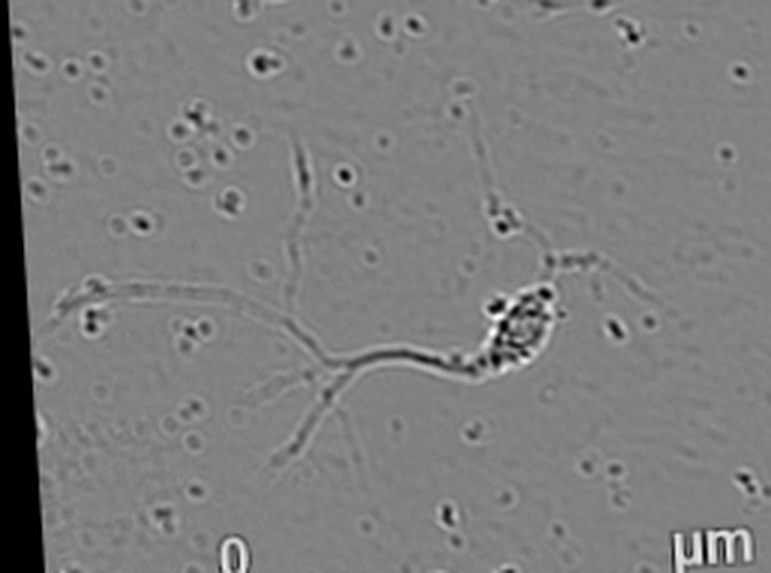
\includegraphics[height=2.2cm,width=2.960cm,keepaspectratio]{fig1_input.png}};
\begin{scope}[on background layer]                 % 3-D stack of frames
  \filldraw[fill=softgrey!55, draw=navy!30]
    ($(raw.south west)+(0.24,0.24)$) rectangle ($(raw.north east)+(0.24,0.24)$);
  \filldraw[fill=softgrey!80, draw=navy!30]
    ($(raw.south west)+(0.12,0.12)$) rectangle ($(raw.north east)+(0.12,0.12)$);
\end{scope}
\draw[draw=navy!45, line width=0.7pt] (raw.south west) rectangle (raw.north east);
\node[plab]   at (1.48,2.55) {(a)~~Time-lapse};
\node[sublab] at (1.48,-0.55) {phase contrast\\$T$ frames};

%------------------------------------------------ (b) annotate frame 0
\node[inner sep=0] (nap) at (5.69,1.0)
     {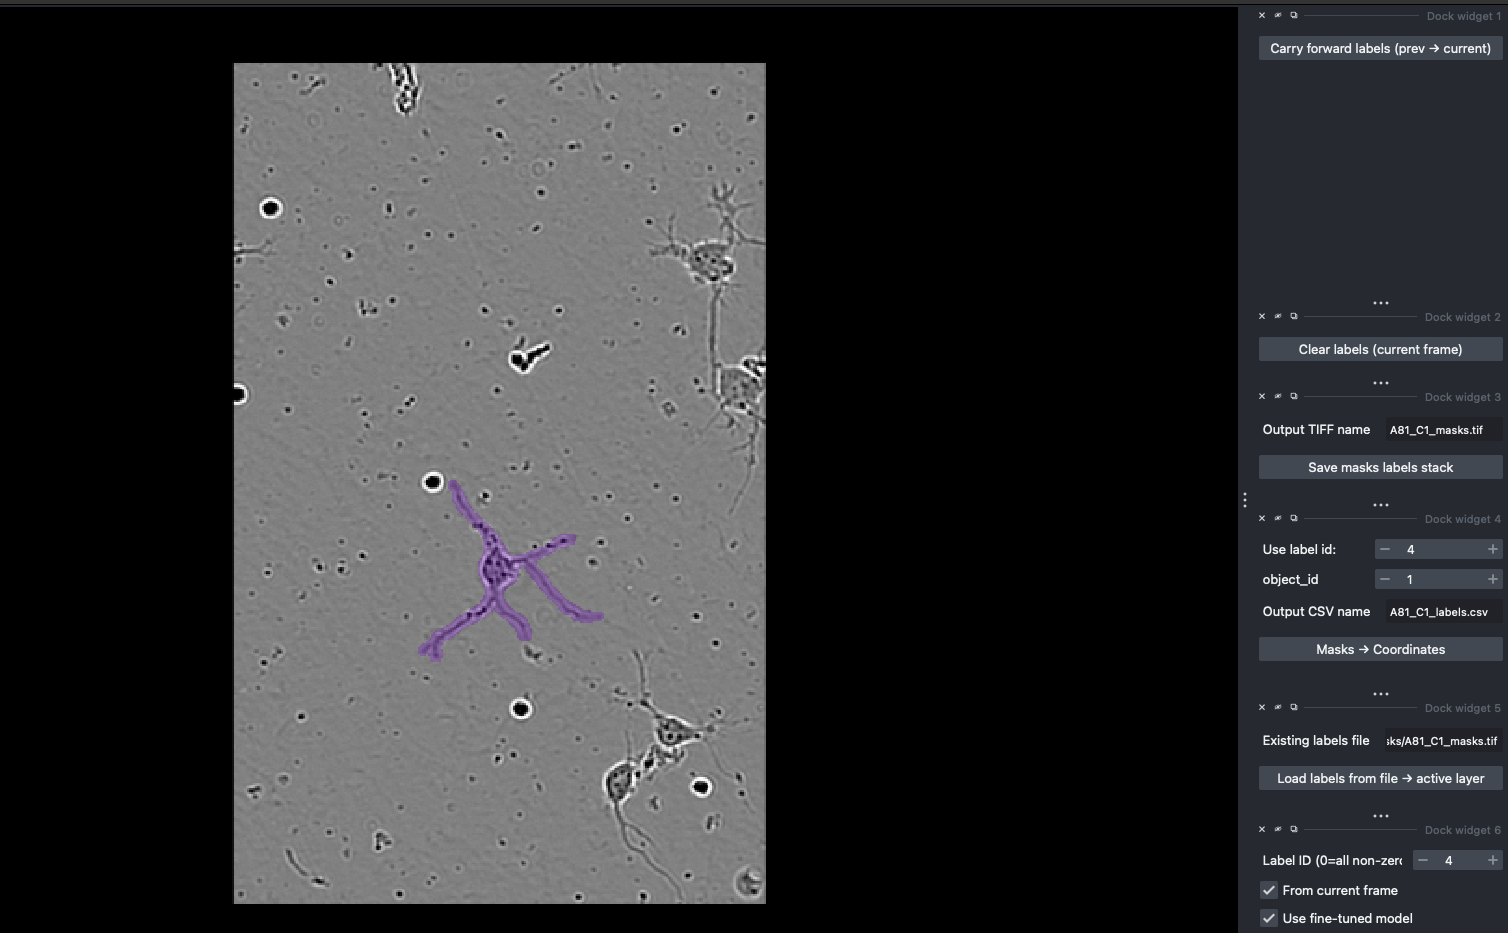
\includegraphics[height=2.2cm,width=3.556cm,keepaspectratio]{fig1_napari.png}};
\draw[draw=amber!85, line width=1pt] (nap.south west) rectangle (nap.north east);
\node[plab]   at (5.69,2.55) {(b)~~Annotate frame 0};
\node[sublab] at (5.69,-0.55) {\texttt{neurons-labeling}\\napari plug-in};

%------------------------------------------------ (c) the model
\node[modelbox] (mdl) at (9.67,1.0)
     {\textbf{Fine-tuned}\\\textbf{SAM\,2}\\[2pt]
      {\scriptsize dual-rank LoRA+}\\[1pt]
      {\scriptsize 13.9\,\% adapted}};
\node[plab]   at (9.67,2.55) {(c)~~Propagate};
\node[sublab] at (9.67,-0.55) {frozen encoder\\$+$ memory attention};

%------------------------------------------------ (d) tracked output
\node[inner sep=0] (res) at (13.35,1.0)
     {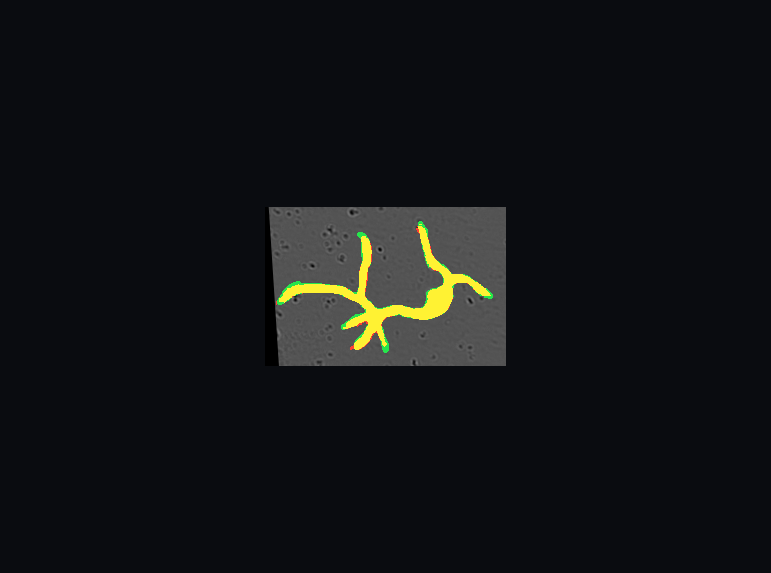
\includegraphics[height=2.2cm,width=2.960cm,keepaspectratio]{fig1_result.png}};
\begin{scope}[on background layer]
  \filldraw[fill=teal!18, draw=teal!45]
    ($(res.south west)+(0.24,0.24)$) rectangle ($(res.north east)+(0.24,0.24)$);
  \filldraw[fill=teal!30, draw=teal!45]
    ($(res.south west)+(0.12,0.12)$) rectangle ($(res.north east)+(0.12,0.12)$);
\end{scope}
\draw[draw=teal!75, line width=0.9pt] (res.south west) rectangle (res.north east);
\node[plab]   at (13.35,2.55) {(d)~~Tracked neuron};
\node[sublab] at (13.35,-0.55) {every frame\\one identity};

%------------------------------------------------ flow
\draw[flowar] (3.06,1.0) -- (3.81,1.0);
\draw[flowar] (7.57,1.0) -- (8.32,1.0);
\draw[flowar] (11.02,1.0) -- (11.77,1.0);

% memory recurrence (model <- its own previous output); routed below the
% sublabel band so it cannot collide with the panel captions
\draw[loopar, draw=teal!85]
  (res.south) .. controls +(0,-1.95) and +(0,-1.95) .. (mdl.south)
  node[midway, below, note, text=teal!75, yshift=-1pt]
  {memory bank $\rightarrow$ next frame};

% human-in-the-loop: corrections become training data
\draw[loopar, draw=amber!90]
  (res.north) .. controls +(0,1.45) and +(0,1.45) .. (nap.north)
  node[midway, above, note, text=amber!85, yshift=1pt]
  {corrections $\rightarrow$ new training data};
\end{tikzpicture}
\caption{\textbf{End-to-end pipeline for single neuron tracking.}
\textbf{(a)}~A continuous label-free phase-contrast time-lapse sequence comprising $T$ frames. \textbf{(b)}~A single target neuron is manually annotated on the initial frame utilizing the integrated \texttt{neurons-labeling} napari plug-in. \textbf{(c)}~The fine-tuned model propagates this spatial prior across the sequence, explicitly maintaining instance identity by conditioning on past predictions via its temporal memory bank. \textbf{(d)}~The target is robustly segmented in every subsequent frame (visualization: true positive in yellow, false negative in green, false positive in red). Interactive corrections made within the plug-in natively generate formatted data for continuous model refinement.}
\label{fig:pipeline}
\end{figure}

%=====================================================================
\section{Related work}
\label{sec:related}

\paragraph{Cell segmentation.} Cell segmentation is dominated by methods
that learn a shape representation and recover instances from it. Cellpose
\cite{stringer2021cellpose} predicts a spatial flow field towards each
cell's center, its SAM-based successor \cite{pachitariu2025cellposesam}
replaces the encoder and extends the training corpus, while StarDist
\cite{schmidt2018stardist} parameterizes instances as star-convex polygons.
Crucially, these U-Net \cite{ronneberger2015unet} descendants intrinsically
assume morphological compactness; this spatial prior is fundamentally
violated by neural processes, which frequently branch or recurve. Omnipose
\cite{cutler2022omnipose} relaxes this constraint by predicting distance
fields relative to object boundaries rather than centroids, making it
geometrically better suited to filamentous structures. However, it remains a
strictly single-frame architecture incapable of longitudinal tracking.
Within our specific modality, NeuroQuantify \cite{chen2024neuroquantify}
effectively segments neurites in phase-contrast microscopy, but it operates
purely as a semantic segmenter lacking instance-level discrimination.
% NeuriteTracker claims verified against the PMC full text (PMC4700477),
% verbatim: "a bicistronic vector that expresses Lifeact-GFP, a fusion of GFP
% with the F-actin binding peptide Lifeact, and a nuclear localization
% NLS-mCherry fusion, which labels the nucleus for cell detection"; "the MSER
% (Maximally Stable Extremal Regions) feature detector followed by a
% morphological filling operation"; "a calibrated Hessian-based filter,
% computing a geodesic distance combining intensity and geometric distance";
% "a graph-association tracking method was applied over the time-lapse data to
% provide a unique label for each tracked cell over time".
NeuriteTracker \cite{fusco2016neuritetracker} aligns most closely with our
task, segmenting neurite morphodynamics across time-lapses and maintaining
instance identity via graph association. However, it relies exclusively on
fluorescence imaging: neurons must express a bicistronic construct carrying
both F-actin and nuclear markers for detection. This invasive labeling is
precisely what continuous, multi-day phase-contrast acquisitions seek to
avoid. Because the pipeline is algorithm-based and specific to fluorescent
markers rather than learned from data, it cannot be trivially adapted to
label-free phase-contrast imagery.

Consequently, when precise, per-neuron morphology is required, the gold
standard remains labor-intensive manual tracing
\cite{meijering2004neuronj,longair2011snt}, as fully automated instance
tracking in this domain remains an open challenge
\cite{liu2022neurontracing}.

\paragraph{Promptable video models and tracking.} The Segment Anything Model
\cite{kirillov2023sam} reconceptualized segmentation as a promptable task,
isolating targets specified via spatial priors such as points, boxes, or
masks. SAM\,2 \cite{ravi2025sam2} extends this paradigm to the video domain
via a memory bank, allowing a single-frame prompt to condition all
subsequent predictions---a foundational mechanism leveraged in this work.
Domain-specific adaptations have built upon this architecture: $\mu$SAM
\cite{archit2025microsam} fine-tunes SAM on microscopy corpora, CellSAM
\cite{israel2025cellsam} integrates an automated detector to eliminate
manual prompting, and SAM\,3 extends the prompting modality from geometric
coordinates to semantic language. While these architectures bring powerful
foundation priors learned at unprecedented scales, none are explicitly
optimized to preserve the topological connectivity of pixel-scale
filamentous structures. Furthermore, temporal identity is conventionally
resolved via a two-stage pipeline---independent spatial segmentation
followed by temporal linking---as standardized by the Cell Tracking
Challenge \cite{maska2023ctc} and implemented in DeepSea
\cite{zargari2023deepsea} and Trackastra \cite{gallusser2024trackastra}.
This separation limits the final result: a tracker cannot recover fine
branches that the segmenter failed to detect. Propagating the mask
continuously through a temporal memory avoids this loss of information,
which is why we adapt a unified video model instead of pairing a segmenter
with a separate tracker.

\paragraph{Topology-preserving objectives and low-rank adaptation.} We
utilize two additional methodologies as foundational components rather than
baselines for comparison. It is well established that area-overlap losses
are insensitive to topological connectivity. Several objectives address this
limitation, including persistent homology \cite{hu2019topology}, clDice
\cite{shit2021cldice} (which penalizes breaks proportionally using soft
skeletons), cbDice \cite{shi2024cbdice} (which applies radius weighting to
prioritize thin branches), and the supervoxel loss \cite{grim2025supervoxel}
(which focuses gradients specifically on structural splits or merges). We
adopt the latter two directly rather than proposing a novel topological
loss. Similarly, we employ established low-rank adaptation techniques (LoRA
\cite{hu2022lora} and LoRA+ \cite{hayou2024loraplus}) without architectural
modification.

Our contribution lies in synthesizing these elements to address a critical
gap. Current shape models lack temporal identity, tracking pipelines inherit
connectivity errors from their segmenters, and video foundation models are
not trained to preserve fine structures. To the best of our knowledge,
topology-preserving objectives have not previously been integrated with
temporal propagation in a promptable video model, nor applied to track
individual neurons in label-free phase-contrast microscopy.

%=====================================================================
\section{Methods}
\label{sec:methods}

\subsection{Data and annotation}
\label{sec:met:data}

\paragraph{Cell culture.}
Primary cortical neurons were isolated from P0--P1 BALB/c mice, dissociated
with papain and plated on poly-D-lysine-coated coverslips at
15{,}625--46{,}875\,cells/cm$^2$ in supplemented Neurobasal medium; the full
protocol is given in \cite{berkovich2025neurite}. Plating densities were
chosen to keep individual neurites optically resolvable rather than to
maximize yield. All procedures were approved by the Bar-Ilan University
Ethics Committee for Animal Research and the Israeli Ministry of Health
(approval no.~43-07-2020).

\paragraph{Live imaging.}
Cultures were imaged in 96-well ImageLock plates on an IncuCyte SX5
Live-Cell Analysis System (Sartorius) with a 10$\times$ objective, acquiring
one phase-contrast frame per hour for 93\,h. Imaging was label-free: no dye
or fluorescent reporter was used, avoiding phototoxicity and
label-induced perturbation across the multi-day acquisition. The spatial
calibration is 1.5\,pixels per micron ($0.667\,\mu$m per pixel).

\paragraph{Recordings.}
Each analyzed recording is a rectangular crop of the full field centered on
one target neuron, so that a single cell and its processes are followed
throughout (Figure~\ref{fig:culture}). Thirty-two recordings were prepared,
spanning 148--615 pixels in width and 146--498 pixels in height
(99--411\,$\mu$m and 98--333\,$\mu$m respectively), and comprising 57--97
frames, most commonly 73. All but one were seeded at the lower of the two
plating densities; \texttt{B28\_C4\_200k} is the single recording at the
higher density, and is included so that the released set is not confined to
one seeding condition. Because a neuron is a thin, branched object within
a much larger field, the target occupies on average 2.5\,\% of the frame,
and as little as 0.2\,\% in the sparsest frames --- the imbalance that
motivates both the loss design (Section~\ref{sec:met:loss}) and the choice
of evaluation metric (Section~\ref{sec:met:metrics}). The fraction is not
constant: it varies by an order of magnitude between recordings (0.9--8.1\,\%
of the frame on average) as neurons of different sizes are followed through
different stages of outgrowth.

\paragraph{Splits.}
Twenty-three recordings were used for training and five for validation and
model selection. Four further recordings --- \texttt{A71\_C1}, \texttt{A81\_C1},
\texttt{A12\_C3\_100k} and \texttt{A12\_C1\_100k\_2} --- were annotated only
after model development was complete and used exclusively as a held-out test
set; the model's weights were never exposed to them. They were selected
simply as the most recently annotated recordings absent from training,
without reference to image quality or segmentation difficulty.

\paragraph{Annotation.}
Ground-truth masks were drawn in \texttt{neurons-labeling}, a napari plug-in
developed for this work and released alongside it
(Figure~\ref{fig:pipeline}b). Annotation followed a human-in-the-loop
protocol: an initial mask was propagated across frames and then corrected
manually. Every mask in the dataset was hand-edited; no propagated output
was accepted unmodified. To confirm that this did not bias evaluation in
favor of the model, we verified that no test-set ground truth coincides
with the model's own prediction: across the 328 scored test frames the
highest agreement is IoU~0.903, with none exceeding 0.95, indicating that
every frame was substantively edited.

\paragraph{The annotation and inference tool.}
\texttt{neurons-labeling} is a napari plug-in, released with this work, that
is both how the dataset was produced and how the model is meant to be used. A
recording is opened as a stack, one neuron is painted on the first frame with
the standard labels brush, and a single action propagates that annotation
through every remaining frame using the weights of
Section~\ref{sec:met:model}; the base SAM\,2 weights can be selected instead,
which is how the zero-shot baseline of Section~\ref{sec:res:benchmark} is
reproduced. Any frame can then be corrected with brush and eraser and the
propagation re-run from that frame. Output is written either as a mask stack
or as a per-pixel coordinate table indexed by frame and object, the form the
downstream morphometric analysis consumes. Because a corrected frame is a
mask in exactly the format the model was trained on, routine use of the tool
produces training data without a separate annotation effort --- the loop drawn
in Figure~\ref{fig:pipeline}.

%---------------------------------------------------------------------
\subsection{Parameter-efficient adaptation of SAM\,2}
\label{sec:met:model}

\paragraph{Backbone.}
We adapt SAM\,2.1 with the Hiera-tiny image encoder
\cite{ravi2025sam2,ryali2023hiera}. SAM\,2 is a promptable \emph{video}
model: it is prompted geometrically --- by a point, box or mask on a single
frame --- and a memory bank carries that prompt forward, so one annotation
can segment an entire recording. The prompt is spatial rather than semantic,
in that the model is told where the object is and not what it is; here we
use a mask prompt on frame~0. Pretrained on SA-V and natural images, SAM\,2
has never encountered phase-contrast microscopy, and its zero-shot behavior
on our recordings is characteristic: it segments the high-contrast soma
reliably and loses the low-contrast processes
(Section~\ref{sec:res:benchmark}). We use the smallest encoder variant, as
with 28 annotated recordings performance is limited by the quantity of
supervision rather than by model capacity.

\paragraph{Input representation.}
Frames are single-channel; each is replicated to three channels, scaled to
$[0,1]$ and resampled to the fixed $1024\times1024$ resolution SAM\,2
expects, with bilinear interpolation for frames and nearest-neighbor
interpolation for masks, preserving hard label boundaries.

As recordings span 192--615 pixels, this resampling is an upsampling by a
factor of 2--5. The encoder emits features at a $16\times$ stride, so a
structure must exceed roughly sixteen input pixels to be represented by more
than a single feature vector; a neurite one to two pixels wide at
acquisition spans four to ten after upsampling and is thereby resolved. The
same consideration governs the input scale chosen for each competing method
(Appendix~\ref{sec:supp:protocol}).

Upsampling introduces no new information and carries two costs. Computation
and memory scale with the resampled area, 3--28 times the native frame. And
because non-square recordings are resampled to a square input rather than
padded, their aspect ratio is altered; we accept this in preference to
padding, which would consume encoder capacity on constant borders, and apply
it identically at training and inference so that the model is never
evaluated under a geometry it did not see.

\paragraph{Adapted and frozen components.}
Adaptation is allocated by parameter mass, so that training remains feasible
on a single GPU. The
image encoder's 27{,}219{,}136 pretrained parameters are frozen in full:
its representations of edges, texture and contrast are generic and were
estimated from a corpus several orders of magnitude larger than ours, and
fine-tuning them on 28 recordings would degrade rather than specialize them.
What must change is not how features are computed but how they are selected,
and that selection happens in attention, where the model determines which
spatial locations and which stored memories bear on the current prediction.
We therefore insert low-rank adapters at 76 attention projections,
distributed across the final two encoder blocks, the memory-attention module
and the mask decoder. These projections are not a separate part of the model
--- they lie within the modules just described --- and their pretrained
weights, 20{,}348{,}928 in total, remain frozen alongside the rest; what is
learned is a low-rank update to each, at a cost of 914{,}432 trainable
parameters, a factor of 22 fewer, with every update confined to a
low-dimensional subspace and thereby regularized. The three sites, whose
counts follow from the architecture, are:

\begin{itemize}\itemsep2pt
  \item \textbf{Memory attention} (40 adapters, rank 16, $\alpha=32$,
        dropout 0.1). Four transformer layers, each comprising a
        self-attention block, a cross-attention block reading from the
        memory bank, and a two-layer feed-forward network --- ten linear
        projections per layer. This module receives the most adaptation; it
        determines how target information is carried between frames.
  \item \textbf{Mask decoder} (28 adapters, rank 16, $\alpha=32$, dropout
        0.1). Two two-way transformer layers, each with self-attention and
        bidirectional token--image cross-attention, giving twelve
        projections per layer, plus a final token-to-image attention
        contributing a further four projections. This module converts
        attended features into the mask, and governs how sharply thin
        structures are delineated.
  \item \textbf{Hiera blocks 10--11} (8 adapters, rank 8, $\alpha=16$).
        The final two blocks of the encoder, contributing per block a fused
        query-key-value projection, an output projection and two
        feed-forward layers. These are the most task-specific layers of the
        encoder, and adapting them at half the rank of the other sites
        permits a limited domain shift without disturbing the frozen
        representation beneath.
\end{itemize}

The non-attention machinery within these same modules --- the mask decoder's
MLP heads, the memory encoder, the prompt encoder and the object-pointer
embeddings, together 4{,}642{,}818 parameters --- is trained without a rank
constraint, since at roughly a fifth of the adapted attention mass little
would be saved by constraining it. In total 34{,}319{,}680 parameters remain
fixed and 5{,}557{,}250 of 39{,}876{,}930 are updated (13.9\,\%);
Figure~\ref{fig:architecture} summarizes the placement.

% ---------------------------------------------------------------------
% Figure 2. Explicit coordinates. Rank labels live INSIDE the boxes so the
% space above the decoder is free for the prompt encoder's arrow.
%   encoder 0.0-2.8 | Hiera 10-11 2.8-4.5 (abutting: same module)
%   memory attention 5.4-8.5 | mask decoder 9.4-12.5 | output arrow to 13.5
%   prompt encoder above the decoder | memory encoder below memory attention
% ---------------------------------------------------------------------
% ============================================================
%  Figure 2 -- method overview.
%  (a) the propagation task   (b) adaptation sites   (c) objective
%  Canvas 16.2 cm = \textwidth (a4paper, 11pt, margin=2.4cm).
%
%  Panel (a) is a raster strip of the real phase-contrast frames of A71_C1
%  (292x292 px, 1.497 px/um) with the frame-0 ground-truth prompt and the
%  shipped model's own propagated masks overlaid -- built by
%  make_filmstrip.py, which re-scores the prediction stack and refuses to
%  draw unless it matches benchmark/results/test/ours_16f.csv.  The
%  acquisition software's burnt-in scale bar and caption are erased from the
%  background there; no pixel of any drawn mask is touched.
%
%  The mask/centerline pair in panel (c) is vector: \neuronTight and
%  \neuronTightSkel below are a marching-squares contour and a
%  skimage skeletonization of the frame-72 ground truth, emitted by
%  trace_masks.py.  Do not hand-edit those paths.
% ============================================================
% ----------------------------------------------------------
% Traced from real ground-truth masks -- training_data/masks/
% Sequence A71_C1, frames [0, 12, 24, 36, 48, 60, 72].  Generated by trace_masks.py;
% do not hand-edit.  Outlines are marching-squares contours of the
% annotated target; the skeleton is skimage.morphology.skeletonize.
% ----------------------------------------------------------
\newcommand{\neuronTight}{%
  \draw[mkfill] (-0.4418,-0.3361) -- (-0.4376,-0.2938) -- (-0.3826,-0.2642) -- (-0.3277,-0.2347) -- (-0.2621,-0.2156) -- (-0.2051,-0.1881) -- (-0.1649,-0.1438) -- (-0.1543,-0.1078) -- (-0.2135,-0.1332) -- (-0.2452,-0.1057) -- (-0.1818,-0.0846) -- (-0.1733,-0.0507) -- (-0.2262,-0.0190) -- (-0.2812,0.0106) -- (-0.3615,0.0148) -- (-0.4418,0.0106) -- (-0.4587,0.0486) -- (-0.3911,0.0486) -- (-0.3234,0.0486) -- (-0.2537,0.0338) -- (-0.1966,0.0063) -- (-0.1818,0.0676) -- (-0.1670,0.1374) -- (-0.1607,0.2072) -- (-0.1290,0.2051) -- (-0.1395,0.1311) -- (-0.1480,0.0550) -- (-0.1628,-0.0106) -- (-0.1205,-0.0528) -- (-0.0550,-0.0507) -- (0.0106,-0.0571) -- (0.0761,-0.0634) -- (0.1163,-0.0190) -- (0.1585,0.0233) -- (0.1628,0.0740) -- (0.1205,0.1163) -- (0.0972,0.1776) -- (0.0761,0.2410) -- (0.0507,0.3002) -- (0.0761,0.3129) -- (0.0994,0.2516) -- (0.1226,0.1903) -- (0.1522,0.1353) -- (0.1966,0.0951) -- (0.2558,0.0698) -- (0.3086,0.0381) -- (0.3573,0.0021) -- (0.4143,-0.0254) -- (0.4630,-0.0528) -- (0.4165,-0.0613) -- (0.3509,-0.0423) -- (0.3065,-0.0021) -- (0.2537,0.0296) -- (0.2072,-0.0042) -- (0.1881,-0.0698) -- (0.1374,-0.1036) -- (0.0698,-0.1205) -- (0.0063,-0.0994) -- (-0.0592,-0.0930) -- (-0.0972,-0.1395) -- (-0.0761,-0.2029) -- (-0.0592,-0.2706) -- (-0.0782,-0.2938) -- (-0.1036,-0.2347) -- (-0.1205,-0.1670) -- (-0.1607,-0.2114) -- (-0.1966,-0.2600) -- (-0.2516,-0.2473) -- (-0.3129,-0.2706) -- (-0.3657,-0.3023) -- (-0.4228,-0.3298);
}
\newcommand{\neuronTightSkel}{%
  \draw[mkskel] (-0.2347,-0.1226) -- (-0.2304,-0.1184) -- (-0.2262,-0.1184) -- (-0.2220,-0.1184) -- (-0.2177,-0.1184) -- (-0.2135,-0.1142) -- (-0.2093,-0.1099) -- (-0.2051,-0.1099) -- (-0.2008,-0.1099) -- (-0.1966,-0.1099) -- (-0.1924,-0.1057) -- (-0.1881,-0.1057) -- (-0.1839,-0.1015) -- (-0.1797,-0.0972) -- (-0.1755,-0.0972) -- (-0.1712,-0.0972) -- (-0.1670,-0.0972) -- (-0.1628,-0.0930) -- (-0.1585,-0.0930) -- (-0.1543,-0.0930) -- (-0.1501,-0.0930) -- (-0.1459,-0.0930) -- (-0.1416,-0.0930) -- (-0.1374,-0.0888) -- (-0.1332,-0.0846) -- (-0.1332,-0.0803) -- (-0.1332,-0.0761) -- (-0.1374,-0.0719) -- (-0.1374,-0.0676) -- (-0.1374,-0.0634) -- (-0.1416,-0.0592) -- (-0.1416,-0.0550) -- (-0.1459,-0.0507) -- (-0.1501,-0.0507) -- (-0.1543,-0.0465) -- (-0.1585,-0.0423) -- (-0.1628,-0.0381) -- (-0.1670,-0.0338) -- (-0.1712,-0.0296) -- (-0.1755,-0.0254) -- (-0.1755,-0.0211) -- (-0.1755,-0.0169) -- (-0.1797,-0.0127) -- (-0.1755,-0.0085) -- (-0.1755,-0.0042) -- (-0.1755,-0.0000) -- (-0.1755,0.0042) -- (-0.1755,0.0085) -- (-0.1755,0.0127) -- (-0.1755,0.0169) -- (-0.1712,0.0211) -- (-0.1712,0.0254) -- (-0.1712,0.0296) -- (-0.1712,0.0338) -- (-0.1712,0.0381) -- (-0.1712,0.0423) -- (-0.1670,0.0465) -- (-0.1670,0.0507) -- (-0.1670,0.0550) -- (-0.1670,0.0592) -- (-0.1670,0.0634) -- (-0.1628,0.0676) -- (-0.1628,0.0719) -- (-0.1628,0.0761) -- (-0.1628,0.0803) -- (-0.1628,0.0846) -- (-0.1628,0.0888) -- (-0.1628,0.0930) -- (-0.1628,0.0972) -- (-0.1628,0.1015) -- (-0.1628,0.1057) -- (-0.1585,0.1099) -- (-0.1585,0.1142) -- (-0.1585,0.1184) -- (-0.1585,0.1226) -- (-0.1543,0.1268) -- (-0.1543,0.1311) -- (-0.1543,0.1353) -- (-0.1501,0.1395) -- (-0.1501,0.1438) -- (-0.1501,0.1480) -- (-0.1501,0.1522) -- (-0.1501,0.1564) -- (-0.1501,0.1607) -- (-0.1459,0.1649) -- (-0.1459,0.1691) -- (-0.1459,0.1733) -- (-0.1459,0.1776) -- (-0.1459,0.1818) -- (-0.1459,0.1860) -- (-0.1459,0.1903) -- (-0.1459,0.1945) -- (-0.1459,0.1987) -- (-0.1459,0.2029) -- (-0.1459,0.2072) -- (-0.1459,0.2114) -- (-0.1459,0.2156);
  \draw[mkskel] (-0.1839,-0.0127) -- (-0.1881,-0.0127) -- (-0.1924,-0.0127) -- (-0.1966,-0.0085) -- (-0.2008,-0.0085) -- (-0.2051,-0.0085) -- (-0.2093,-0.0085) -- (-0.2135,-0.0042) -- (-0.2177,-0.0000) -- (-0.2220,-0.0000) -- (-0.2262,0.0042) -- (-0.2304,0.0042) -- (-0.2347,0.0085) -- (-0.2389,0.0085) -- (-0.2431,0.0127) -- (-0.2473,0.0127) -- (-0.2516,0.0169) -- (-0.2558,0.0211) -- (-0.2600,0.0211) -- (-0.2642,0.0211) -- (-0.2685,0.0254) -- (-0.2727,0.0254) -- (-0.2769,0.0254) -- (-0.2812,0.0296) -- (-0.2854,0.0296) -- (-0.2896,0.0296) -- (-0.2938,0.0296) -- (-0.2981,0.0296) -- (-0.3023,0.0296) -- (-0.3065,0.0296) -- (-0.3108,0.0338) -- (-0.3150,0.0338) -- (-0.3192,0.0338) -- (-0.3234,0.0338) -- (-0.3277,0.0338) -- (-0.3319,0.0338) -- (-0.3361,0.0338) -- (-0.3404,0.0338) -- (-0.3446,0.0338) -- (-0.3488,0.0338) -- (-0.3530,0.0338) -- (-0.3573,0.0338) -- (-0.3615,0.0338) -- (-0.3657,0.0338) -- (-0.3699,0.0338) -- (-0.3742,0.0338) -- (-0.3784,0.0296) -- (-0.3826,0.0296) -- (-0.3869,0.0296) -- (-0.3911,0.0296) -- (-0.3953,0.0296) -- (-0.3995,0.0296) -- (-0.4038,0.0296) -- (-0.4080,0.0296) -- (-0.4122,0.0296) -- (-0.4165,0.0296) -- (-0.4207,0.0296) -- (-0.4249,0.0296) -- (-0.4291,0.0296) -- (-0.4334,0.0296) -- (-0.4376,0.0296) -- (-0.4418,0.0296);
  \draw[mkskel] (-0.1290,-0.0846) -- (-0.1205,-0.0846) -- (-0.1120,-0.0846) -- (-0.1036,-0.0846) -- (-0.0951,-0.0803) -- (-0.0867,-0.0803) -- (-0.0782,-0.0761) -- (-0.0698,-0.0761) -- (-0.0613,-0.0719) -- (-0.0528,-0.0719) -- (-0.0444,-0.0676) -- (-0.0359,-0.0676) -- (-0.0275,-0.0676) -- (-0.0190,-0.0676) -- (-0.0106,-0.0719) -- (-0.0021,-0.0719) -- (0.0063,-0.0761) -- (0.0148,-0.0803) -- (0.0233,-0.0803) -- (0.0317,-0.0846) -- (0.0402,-0.0888) -- (0.0486,-0.0888) -- (0.0571,-0.0930) -- (0.0655,-0.0930) -- (0.0740,-0.0930) -- (0.0824,-0.0930) -- (0.0909,-0.0888) -- (0.0994,-0.0888) -- (0.1078,-0.0803) -- (0.1163,-0.0761) -- (0.1247,-0.0719) -- (0.1332,-0.0634) -- (0.1416,-0.0550) -- (0.1501,-0.0465) -- (0.1585,-0.0381) -- (0.1628,-0.0296) -- (0.1712,-0.0211) -- (0.1755,-0.0127) -- (0.1797,-0.0042) -- (0.1797,0.0042) -- (0.1881,0.0127) -- (0.1881,0.0211) -- (0.1881,0.0296) -- (0.1924,0.0381) -- (0.1966,0.0465) -- (0.1924,0.0550) -- (0.1924,0.0634) -- (0.1881,0.0719) -- (0.1839,0.0803) -- (0.1755,0.0888) -- (0.1670,0.0972) -- (0.1585,0.1057) -- (0.1501,0.1099) -- (0.1416,0.1184) -- (0.1332,0.1268) -- (0.1290,0.1353) -- (0.1247,0.1438) -- (0.1205,0.1522) -- (0.1163,0.1607) -- (0.1120,0.1691) -- (0.1120,0.1776) -- (0.1078,0.1860) -- (0.1036,0.1945) -- (0.1036,0.2029) -- (0.0994,0.2114) -- (0.0994,0.2199) -- (0.0951,0.2283) -- (0.0909,0.2368) -- (0.0867,0.2452) -- (0.0824,0.2537) -- (0.0782,0.2621) -- (0.0698,0.2706) -- (0.0655,0.2790) -- (0.0655,0.2875) -- (0.0655,0.2960) -- (0.0613,0.3044) -- (0.0655,0.3129) -- (0.0655,0.3213);
  \draw[mkskel] (0.2008,0.0507) -- (0.2051,0.0507) -- (0.2093,0.0507) -- (0.2135,0.0507) -- (0.2177,0.0507) -- (0.2220,0.0507) -- (0.2262,0.0507) -- (0.2304,0.0507) -- (0.2347,0.0507) -- (0.2389,0.0507) -- (0.2431,0.0507) -- (0.2473,0.0507) -- (0.2516,0.0507) -- (0.2558,0.0465) -- (0.2600,0.0465) -- (0.2642,0.0465) -- (0.2685,0.0423) -- (0.2727,0.0423) -- (0.2769,0.0423) -- (0.2812,0.0423) -- (0.2854,0.0381) -- (0.2896,0.0338) -- (0.2938,0.0296) -- (0.2981,0.0254) -- (0.3023,0.0254) -- (0.3065,0.0211) -- (0.3108,0.0169) -- (0.3150,0.0127) -- (0.3192,0.0085) -- (0.3234,0.0042) -- (0.3277,-0.0000) -- (0.3319,-0.0042) -- (0.3361,-0.0042) -- (0.3404,-0.0085) -- (0.3446,-0.0085) -- (0.3488,-0.0127) -- (0.3530,-0.0169) -- (0.3573,-0.0211) -- (0.3615,-0.0254) -- (0.3657,-0.0296) -- (0.3699,-0.0296) -- (0.3742,-0.0338) -- (0.3784,-0.0338) -- (0.3826,-0.0338) -- (0.3869,-0.0381) -- (0.3911,-0.0381) -- (0.3953,-0.0381) -- (0.3995,-0.0381) -- (0.4038,-0.0381) -- (0.4080,-0.0381) -- (0.4122,-0.0423) -- (0.4165,-0.0423) -- (0.4207,-0.0423) -- (0.4249,-0.0465) -- (0.4291,-0.0465) -- (0.4334,-0.0465) -- (0.4376,-0.0507) -- (0.4418,-0.0550) -- (0.4461,-0.0550) -- (0.4503,-0.0592) -- (0.4545,-0.0592);
  \draw[mkskel] (-0.1120,-0.0888) -- (-0.1120,-0.0930) -- (-0.1120,-0.0972) -- (-0.1163,-0.1015) -- (-0.1163,-0.1057) -- (-0.1163,-0.1099) -- (-0.1163,-0.1142) -- (-0.1163,-0.1184) -- (-0.1163,-0.1226) -- (-0.1163,-0.1268) -- (-0.1163,-0.1311) -- (-0.1205,-0.1353) -- (-0.1205,-0.1395) -- (-0.1205,-0.1438) -- (-0.1247,-0.1480) -- (-0.1290,-0.1480) -- (-0.1332,-0.1480) -- (-0.1374,-0.1522) -- (-0.1416,-0.1522) -- (-0.1459,-0.1564) -- (-0.1501,-0.1607) -- (-0.1501,-0.1649) -- (-0.1543,-0.1691) -- (-0.1585,-0.1733) -- (-0.1585,-0.1776) -- (-0.1628,-0.1818) -- (-0.1670,-0.1860) -- (-0.1712,-0.1903) -- (-0.1755,-0.1945) -- (-0.1797,-0.1987) -- (-0.1839,-0.2029) -- (-0.1881,-0.2072) -- (-0.1881,-0.2114) -- (-0.1924,-0.2156) -- (-0.1966,-0.2199) -- (-0.2008,-0.2199) -- (-0.2051,-0.2199) -- (-0.2093,-0.2199) -- (-0.2135,-0.2199) -- (-0.2177,-0.2199) -- (-0.2220,-0.2241) -- (-0.2262,-0.2241) -- (-0.2304,-0.2241) -- (-0.2347,-0.2241) -- (-0.2389,-0.2241) -- (-0.2431,-0.2241) -- (-0.2473,-0.2241) -- (-0.2516,-0.2283) -- (-0.2558,-0.2283) -- (-0.2600,-0.2283) -- (-0.2642,-0.2325) -- (-0.2685,-0.2325) -- (-0.2727,-0.2368) -- (-0.2769,-0.2368) -- (-0.2812,-0.2368) -- (-0.2854,-0.2410) -- (-0.2896,-0.2410) -- (-0.2938,-0.2410) -- (-0.2981,-0.2410) -- (-0.3023,-0.2452) -- (-0.3065,-0.2452) -- (-0.3108,-0.2495) -- (-0.3150,-0.2495) -- (-0.3192,-0.2537) -- (-0.3234,-0.2537) -- (-0.3277,-0.2579) -- (-0.3319,-0.2579) -- (-0.3361,-0.2621) -- (-0.3404,-0.2621) -- (-0.3446,-0.2664) -- (-0.3488,-0.2706) -- (-0.3530,-0.2706) -- (-0.3573,-0.2748) -- (-0.3615,-0.2748) -- (-0.3657,-0.2790) -- (-0.3699,-0.2833) -- (-0.3742,-0.2833) -- (-0.3784,-0.2875) -- (-0.3826,-0.2875) -- (-0.3869,-0.2875) -- (-0.3911,-0.2875) -- (-0.3953,-0.2917) -- (-0.3995,-0.2917) -- (-0.4038,-0.2917) -- (-0.4080,-0.2960) -- (-0.4122,-0.3002) -- (-0.4165,-0.3044) -- (-0.4207,-0.3044) -- (-0.4249,-0.3086) -- (-0.4291,-0.3129) -- (-0.4334,-0.3171) -- (-0.4376,-0.3213) -- (-0.4418,-0.3213) -- (-0.4461,-0.3256);
  \draw[mkskel] (-0.1205,-0.1480) -- (-0.1163,-0.1522) -- (-0.1120,-0.1564) -- (-0.1078,-0.1564) -- (-0.1036,-0.1607) -- (-0.1036,-0.1649) -- (-0.1036,-0.1691) -- (-0.1036,-0.1733) -- (-0.0994,-0.1776) -- (-0.0994,-0.1818) -- (-0.0994,-0.1860) -- (-0.0994,-0.1903) -- (-0.0951,-0.1945) -- (-0.0951,-0.1987) -- (-0.0951,-0.2029) -- (-0.0951,-0.2072) -- (-0.0909,-0.2114) -- (-0.0909,-0.2156) -- (-0.0909,-0.2199) -- (-0.0867,-0.2241) -- (-0.0867,-0.2283) -- (-0.0867,-0.2325) -- (-0.0824,-0.2368) -- (-0.0824,-0.2410) -- (-0.0824,-0.2452) -- (-0.0782,-0.2495) -- (-0.0782,-0.2537) -- (-0.0782,-0.2579) -- (-0.0782,-0.2621) -- (-0.0740,-0.2664) -- (-0.0740,-0.2706) -- (-0.0698,-0.2748) -- (-0.0698,-0.2790) -- (-0.0698,-0.2833) -- (-0.0655,-0.2875) -- (-0.0655,-0.2917) -- (-0.0613,-0.2960) -- (-0.0613,-0.3002) -- (-0.0613,-0.3044);
}
% skeleton 513 px vs 4977 mask px -> skeleton is 10.3\% of the mask

% framed panel holding a traced mask: #1 x, #2 y, #3 half-size, #4 macro
\newcommand{\maskpanel}[4]{%
  \begin{scope}[shift={(#1,#2)}]
    \draw[black!35, line width=0.35pt, fill=white] (-#3,-#3) rectangle (#3,#3);
    \begin{scope}[scale={2*#3}]#4\end{scope}
  \end{scope}
}

\begin{figure}[!htb]
\centering
\begin{tikzpicture}[
  font=\small,
  rule/.style={draw=black!45, line width=0.4pt},
  plab/.style={font=\bfseries\small, text=black, anchor=north west},
  ptit/.style={font=\small, text=black, anchor=north west},
  note/.style={font=\scriptsize, text=black!60, align=left},
  sm/.style={font=\fontsize{6.4}{7.4}\selectfont, text=black!60},
  bx/.style={rounded corners=1pt, align=center, inner sep=2.5pt,
             line width=0.5pt, font=\fontsize{7}{8}\selectfont},
  frz/.style={bx, fill=black!5,    draw=black!45},
  lra/.style={bx, fill=ourblue!10, draw=ourblue!75},
  trn/.style={bx, fill=teal!10,    draw=teal!75},
  ar/.style={-{Stealth[length=1.7mm,width=1.4mm]}, draw=black!65, line width=0.5pt},
  loop/.style={-{Stealth[length=1.7mm,width=1.4mm]}, draw=amber!85!black,
               line width=0.7pt},
  grad/.style={-{Stealth[length=1.7mm,width=1.4mm]}, draw=crimson!85,
               line width=0.6pt},
  mkfill/.style={fill=mk!25, draw=mk!90!black, line width=0.25pt},
  mkskel/.style={draw=mk2, line width=0.4pt, line cap=round},
  nd/.style={circle, draw=black!60, fill=white, line width=0.5pt,
             minimum size=0.26cm, inner sep=0pt},
]

% ==================  (a)  the propagation task  ==================
\node[plab] at (0.00,7.55) {(a)};
\node[ptit] at (0.62,7.55)
     {One annotation at $t=0$ propagates through the whole recording};
\node[note, anchor=north east] at (16.20,7.55)
     {target area $1.5\,\% \rightarrow 5.8\,\%$ of the frame};

% Real phase contrast: the frame-0 ground-truth prompt (navy) and the model's
% own propagated masks (teal).  Seven 1.24 cm cells on a 2.30 cm pitch, 50 um
% scale bar burnt into the last cell.  Built by make_filmstrip.py, which
% refuses to draw unless the stack re-scores to the IoU in ours_16f.csv.
\node[anchor=south west, inner sep=0] at (0.53,5.80)
     {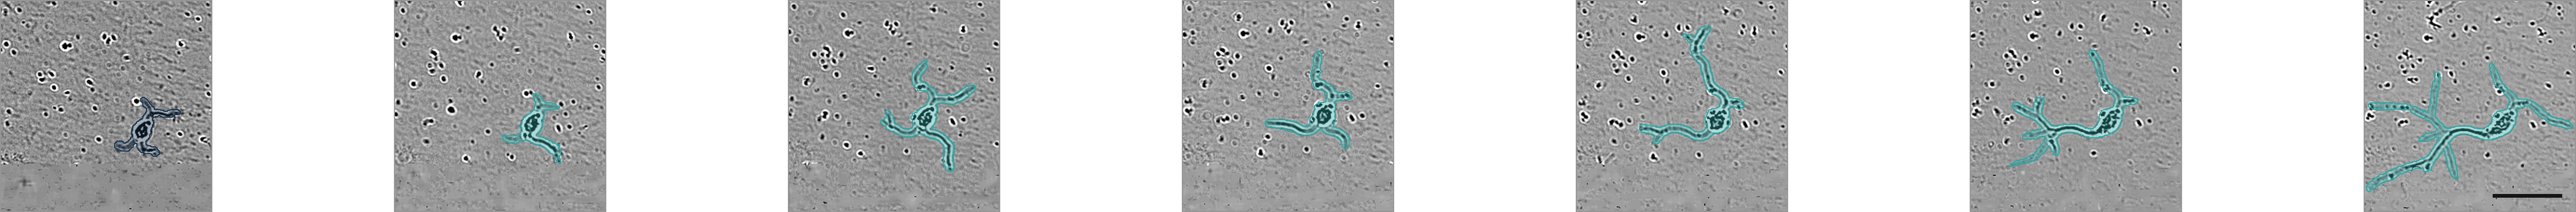
\includegraphics[width=15.04cm]{fig2_filmstrip}};

\draw[rule] (0.90,5.70) -- (15.35,5.70);
\foreach \x in {1.15,3.45,5.75,8.05,10.35,12.65,14.95}
  \draw[rule] (\x,5.70) -- (\x,5.60);
\foreach \x/\lb in {1.15/0, 3.45/12, 5.75/24, 8.05/36, 10.35/48, 12.65/60,
                    14.95/72}
  \node[sm, anchor=north] at (\x,5.56) {\lb};
\node[sm, anchor=west] at (15.45,5.64) {h};
\node[sm, text=navy, anchor=north] at (1.15,5.26) {given};
\node[sm, anchor=north east] at (16.20,5.26) {scale bar $50\,\mu$m};
\node[sm, anchor=north] at (9.20,5.26)
     {propagated with no further prompt, correction or re-initialization};

\draw[rule] (0,4.88) -- (16.20,4.88);

% ==================  (b)  where the model is adapted  ============
\node[plab] at (0.00,4.68) {(b)};
\node[ptit] at (0.62,4.68) {Adaptation sites};
\node[note, anchor=north west] at (0.62,4.32)
     {$5{,}557{,}250$ of $39{,}876{,}930$ parameters updated ($13.9\,\%$)};

\node[frz, minimum width=2.30cm, minimum height=0.74cm, anchor=west] (enc)
     at (0.10,3.35) {Image encoder\\{\fontsize{6}{7}\selectfont Hiera-tiny}};
\node[lra, minimum width=1.70cm, minimum height=0.74cm, anchor=west] (hier)
     at (2.85,3.35) {blocks 10--11\\{\fontsize{6}{7}\selectfont $r{=}8$}};
\node[trn, minimum width=2.10cm, minimum height=0.74cm, anchor=west] (pe)
     at (6.10,3.35) {Prompt encoder\\{\fontsize{6}{7}\selectfont frame-0 mask}};

\node[lra, minimum width=2.55cm, minimum height=0.80cm, anchor=west] (mem)
     at (0.10,1.95) {Memory attention\\{\fontsize{6}{7}\selectfont $r{=}16$,
       40 sites}};
\node[lra, minimum width=2.55cm, minimum height=0.80cm, anchor=west] (dec)
     at (3.30,1.95) {Mask decoder\\{\fontsize{6}{7}\selectfont $r{=}16$,
       28 sites}};
\node[trn, minimum width=2.90cm, minimum height=0.50cm, anchor=west] (menc)
     at (2.00,0.72) {Memory encoder $+$ bank};

\draw[ar] (enc.east) -- (hier.west);
\draw[ar] (hier.south) -- ++(0,-0.26) -| (mem.north);
\draw[ar] (mem.east) -- (dec.west);
\draw[ar] (pe.south) -- ++(0,-0.42) -| ([xshift=8mm]dec.north);
\draw[ar] (dec.east) -- ++(0.24,0) node[right, sm, text=black] {$\hat{m}_t$};
\draw[loop] (dec.south) -- (dec.south |- menc.north);
\draw[loop] (menc.west) -| (mem.south);
\node[sm, text=amber!55!black, anchor=west] at (0.10,0.18)
     {the bank read at $t$ holds the mask predicted at $t-1$};

% --- key
\begin{scope}[shift={(0.10,-0.30)}]
  \node[frz, minimum width=0.26cm, minimum height=0.17cm, anchor=west] at (0,0) {};
  \node[sm, anchor=west, text=black] at (0.32,0) {frozen};
  \node[lra, minimum width=0.26cm, minimum height=0.17cm, anchor=west] at (1.25,0) {};
  \node[sm, anchor=west, text=black] at (1.57,0) {LoRA-adapted, $0.91$\,M};
  \node[trn, minimum width=0.26cm, minimum height=0.17cm, anchor=west] at (4.45,0) {};
  \node[sm, anchor=west, text=black] at (4.77,0) {trained directly, $4.64$\,M};
\end{scope}

% ==================  (c)  the objective  =========================
\draw[rule] (9.10,4.68) -- (9.10,-0.50);

\node[plab] at (9.35,4.68) {(c)};
\node[ptit] at (9.97,4.68) {Objective};
\node[note, anchor=north west] at (9.97,4.32)
     {16-frame clips, bank not detached};

\node[sm, anchor=south] at (12.40,3.58) {memory writes};
\node[nd] (n0) at (10.15,3.42) {};
\node[nd] (n1) at (11.35,3.42) {};
\node[nd] (n2) at (12.55,3.42) {};
\node[nd] (n3) at (14.75,3.42) {};
\node[sm] at (13.65,3.42) {$\cdots$};
\draw[ar] (n0) -- (n1);
\draw[ar] (n1) -- (n2);
\draw[ar] (n2) -- (13.30,3.42);
\draw[ar] (14.00,3.42) -- (n3);
\foreach \x/\lb in {10.15/t, 11.35/{t{+}1}, 12.55/{t{+}2}, 14.75/{t{+}15}}
  \node[sm, anchor=north] at (\x,3.18) {$\lb$};

\draw[grad] (14.75,2.92) .. controls (13.80,2.46) and (11.10,2.46) .. (10.15,2.92);
\node[sm, text=crimson!85, anchor=north] at (12.45,2.50)
     {gradient retained back to the start of the clip};

% --- the composite loss, as a ruled table
\draw[rule] (9.35,2.02) -- (16.20,2.02);
\node[sm, anchor=west] at (9.42,1.86) {weight};
\node[sm, anchor=west] at (10.42,1.86) {term};
\node[sm, anchor=west] at (12.30,1.86) {compares};
\draw[rule] (9.35,1.72) -- (16.20,1.72);
\foreach \y/\w/\t/\c in {1.52/{$3.0$}/{Focal}/{pixels},
                         1.22/{$2.0$}/{Dice}/{regions}}{
  \node[font=\fontsize{6.8}{7.8}\selectfont, anchor=west] at (9.42,\y) {\w};
  \node[font=\fontsize{6.8}{7.8}\selectfont, anchor=west] at (10.42,\y) {\t};
  \node[sm, anchor=west] at (12.30,\y) {\c};
}
\foreach \y/\w/\t/\c in {0.92/{$0.3$}/{cbDice}/{centerlines},
                         0.62/{$0.3$}/{Supervoxel}/{connected components}}{
  \node[font=\fontsize{6.8}{7.8}\selectfont, text=ourblue, anchor=west] at (9.42,\y) {\w};
  \node[font=\fontsize{6.8}{7.8}\selectfont, text=ourblue, anchor=west] at (10.42,\y) {\t};
  \node[sm, text=ourblue!85!black, anchor=west] at (12.30,\y) {\c};
}
\draw[rule] (9.35,0.44) -- (16.20,0.44);

% --- what the two topology terms actually look at
\colorlet{mk}{black!45}\colorlet{mk2}{ourblue}
\maskpanel{9.78}{-0.06}{0.36}{\neuronTight\neuronTightSkel}
\node[sm, anchor=west, align=left] at (10.30,-0.06)
     {the centerline is $513$ of the mask's $4977$ pixels:\\
      a severed branch barely moves an area term};

\end{tikzpicture}
\caption{\textbf{Methodology and architectural adaptation.}
\textbf{(a) The task:} Conditioned exclusively on a single ground-truth mask at $t=0$ (navy), the model autonomously propagates predictions (teal) longitudinally without secondary prompting.
\textbf{(b) Parameter-efficient adaptation:} The Hiera-tiny image encoder is frozen except for low-rank adapters ($r{=}8$) in its final two blocks, while rank-16 adapters are integrated into the memory-attention and mask decoders alongside fully fine-tuned prompt and memory encoders (the amber pathway illustrates temporal recurrence, Eq.~\ref{eq:recurrence}).
\textbf{(c) Optimization and temporal backpropagation:} By maintaining the memory bank within the computation graph across unrolled 16-frame training clips, gradients continuously optimize cross-frame parameters, while topology-aware loss terms explicitly penalize structural fractures.}
\label{fig:architecture}
\end{figure}


\paragraph{Low-rank adaptation.}
For a frozen weight matrix
$W_0 \in \mathbb{R}^{d_{\text{out}} \times d_{\text{in}}}$ the update is
constrained to a rank-$r$ subspace and only $A$ and $B$ are trained,
\begin{equation}
W = W_0 + \frac{\alpha}{r}\,BA,
\qquad
A \in \mathbb{R}^{r \times d_{\text{in}}},\;
B \in \mathbb{R}^{d_{\text{out}} \times r},\;
r \ll \min(d_{\text{in}}, d_{\text{out}}).
\label{eq:lora}
\end{equation}
The per-layer cost falls from $d_{\text{out}}d_{\text{in}}$ to
$r(d_{\text{in}}+d_{\text{out}})$ parameters --- for the 256-dimensional
projections that dominate our adapted layers, from 65{,}536 to 8{,}192 at
$r=16$. The rank is as much a capacity constraint as an efficiency measure:
it confines the update to $r$ directions and so regularizes adaptation where
supervision is scarce, which is why we use $r=16$ where substantial change
is required and $r=8$ within the encoder, where only a bounded shift is
intended. $A$ is initialized Kaiming-uniform and $B$ to zero, so
$\Delta W = 0$ at initialization and optimization begins at the pretrained
model; the $\alpha/r$ scaling decouples update magnitude from $r$.

Zero-initialization induces an optimization asymmetry:
$\partial\mathcal{L}/\partial A \propto \lVert B \rVert$ vanishes at the
first step while $\partial\mathcal{L}/\partial B$ does not, so a shared
learning rate advances the two factors at systematically different rates.
LoRA+ \cite{hayou2024loraplus} assigns them separate rates,
$\mathrm{lr}_B = \lambda\,\mathrm{lr}_A$, which is feature-learning optimal
in the large-width limit; we take $\lambda = 16$
($\mathrm{lr}_A = 1\times10^{-4}$, $\mathrm{lr}_B = 1.6\times10^{-3}$).
Directly-trained modules use $1\times10^{-5}$, as they carry pretrained
structure sensitive to large updates.

\paragraph{Propagation and gradient flow.}
SAM\,2 processes a recording sequentially, maintaining a memory bank that
summarizes what has been observed. Writing $I_t$ for the frame at time $t$,
$E$ for the frozen encoder and $M_t$ for the bank after frame $t$ has been
processed, each step comprises attending to the past, predicting the mask,
and storing the result:
\begin{equation}
F_t = \mathrm{MemAttn}\!\big(E(I_t),\, M_{t-1}\big),
\qquad
\hat{m}_t = \mathrm{Dec}(F_t),
\qquad
M_t = \big[\, M_{t-1};\; \mathrm{MemEnc}(I_t, \hat{m}_t) \,\big],
\label{eq:recurrence}
\end{equation}
with $M_0$ formed from the frame-0 prompt. The third operation renders the
system recurrent: the bank consumed at step $t$ contains the mask predicted
at step $t-1$, so the prediction at any frame is a function of every
prediction preceding it.

The consequence for training is that the gradient of the loss at a given
frame reaches the adapters along paths of increasing length --- one through
the current frame, one through the previous frame's memory write, and so on
to the beginning of the clip --- and retaining these paths requires that the
bank not be detached from the computation graph between frames. Many
implementations do detach it, which reduces training memory and simplifies
the backward pass; we do not. The distinction is consequential because the
parameters that govern cross-frame behavior --- the 40 memory-attention
adapters and the memory encoder --- receive gradient only along the paths
that detachment removes. Under detachment they would be optimized as though
the frames were independent, yielding a model that segments frames rather
than one that propagates a mask. Training accordingly proceeds by
backpropagation through time over clips of 16 frames, each with a single
conditioning frame, which bounds the length of the retained paths and hence
the memory cost.

\paragraph{Inference.}
The same recurrence runs at test time without gradients. The ground-truth
mask of frame~0 is passed directly to the output and into the memory bank,
and the recording is then propagated in full --- 57 to 93 frames --- rather
than in the sixteen-frame clips used for training and validation, with no
further prompt, correction or re-initialization. Preprocessing is the validation transform
above, without augmentation; output logits are thresholded at zero and
resampled to the native resolution of the recording by nearest-neighbor
interpolation.



\subsection{Topology-preserving loss}
\label{sec:met:loss}

\paragraph{Motivation.}
Two properties of neuronal morphology make our recordings difficult to
segment: branches can be only a few pixels wide, and neighboring branches
often touch or overlap due to the image resolution
\cite{grim2025supervoxel}. An error at this scale --- negligible under a
per-pixel or region-overlap loss --- can therefore split one branch into
two, or merge two branches into one. The loss score is almost unchanged, yet
the reconstructed morphology is no longer usable for the measurements that
motivate the segmentation.

Splits and merges are topological errors: they change the connectivity of
the segmented neuron while leaving its area essentially intact, and neither
a per-pixel nor a region-overlap term can register them. We therefore
include two terms that operate on topology. cbDice \cite{shi2024cbdice}
compares the centerlines of prediction and target rather than their areas,
and weights that comparison by local thickness so that a thin branch counts
more than the cell body --- exactly where an area-based loss is weakest. The
supervoxel loss \cite{grim2025supervoxel} examines the connected components
of the error mask and identifies those whose addition or removal would
change the number of connected components in the prediction; it penalizes
false splits and false merges directly, which cbDice, comparing centerlines,
does not.

\paragraph{The composite loss.}
% NOTE: loss_iou and loss_class are identically 0.000000 in every logged
% epoch of both checkpoints/ and checkpoints-16-frames/. They are gated on
% pred_obj_scores, which the training wrapper does not emit, so the loss
% actually optimized has FOUR terms. This is a property of the wrapper, not
% of any one run. Do not reinstate the six-term form.
We supervise the predicted mask with a weighted sum of four terms against the
ground truth --- two that measure agreement in the conventional way, per pixel
and per region, and two that measure topology --- together with two further
terms against a privileged teacher, introduced below:
\begin{equation}
\mathcal{L} = \underbrace{3\,\mathcal{L}_{\text{focal}}
 + 2\,\mathcal{L}_{\text{Dice}}
 + 0.3\,\mathcal{L}_{\text{cbDice}}
 + 0.3\,\mathcal{L}_{\text{sv}}}_{\text{against the ground truth}}
 + \underbrace{0.2\,\mathcal{L}^{\,T}_{\text{Dice}}
 + 0.1\,\mathcal{L}^{\,T}_{\text{cbDice}}}_{\text{against the teacher}} .
\label{eq:loss}
\end{equation}
The first four terms are described in this section; the superscript-$T$ terms
are defined in the paragraph on distillation below, and are zero for the
frames on which no teacher is decoded.
The first two terms are the mask supervision under which SAM and SAM\,2 were
trained \cite{kirillov2023sam,ravi2025sam2}; we keep it so that adaptation
proceeds under the same supervision that produced the pretrained weights,
and retune only the relative weights. The Focal loss term
\cite{lin2017focal} is a cross-entropy in which every pixel is scaled by a
class factor $\alpha_t$ and by $(1-p_t)^{\gamma}$, so that a pixel already
classified confidently contributes almost nothing; we use the standard
pairing $\gamma = 2.0$, $\alpha = 0.25$, the focusing term having already
absorbed most of the imbalance that $\alpha$ would otherwise correct. The
target is a small share of each frame and that share varies by an order of
magnitude across recordings, so an unweighted cross-entropy would be
dominated by background the model classifies correctly from the first epoch,
while a fixed class weight would have to be retuned per recording. The focal
term instead adapts pixel by pixel, redirecting capacity to those that
remain ambiguous --- here the branch boundaries and the lowest-contrast
neurites. The Dice term \cite{milletari2016vnet} compares the two masks as
regions and normalizes by their combined area, which makes it independent of
how much of the frame the neuron occupies and supplies a gradient that
depends on the mask as a whole rather than on pixels independently --- both
properties that the per-pixel term lacks. The four terms therefore act on
pixels, regions, skeletons and connected components respectively.
\paragraph{Centerline-boundary Dice.}
cbDice \cite{shi2024cbdice} extends clDice \cite{shit2021cldice}, which
compares the skeletons of prediction and target rather than their masks: a
skeleton holds far fewer pixels than the region it summarizes, so a break
that is negligible in area removes a visible fraction of it. cbDice adds
scale, weighting each centerline pixel by the local thickness of the
structure it belongs to. We follow clDice's notation: $V_P$ is the predicted
mask, $V_L$ the binary ground truth, and $S_P$, $S_L$ their skeletons.

% Eq. (4)-(7) verified line-by-line against src/loss_fns.py after commits
% d4edf6c (faithful port of reference cbDice + clDice seed) and a3cdc39
% (cbDice weight 5.0 -> 1.0). I_N is the "subtraction-based inverse" that is
% the active branch of get_weights() in the authors' reference code
% (github.com/PengchengShi1220/cbDice); they also ship a commented-out
% "division-based" variant, R_max/R, which is what their paper's prose
% describes. Re-check if loss_fns.py changes again.
We build a differentiable skeleton by iterative morphological opening --- an
erosion followed by a dilation, implemented as min- and max-pooling over the
four-connected cross and the $3\times3$ square respectively, akin to clDice.
Opening shrinks a shape and regrows it, but what the erosion destroys cannot
be regrown. For a given mask $I$, the difference $I - \mathrm{open}(I)$
extracts its thin structure, while applying this iteratively to the eroded
mask reveals progressively thicker formations. Letting $I_k$ denote the mask
after $k$ erosions,
$\delta_k = \mathrm{ReLU}\big(I_k - \mathrm{open}(I_k)\big)$ the structure
it exposes, and $S_k$ the accumulated skeleton,
\begin{equation}
S_k = S_{k-1} + \mathrm{ReLU}\big(\delta_k - S_{k-1}\,\delta_k\big),
\qquad
\mathrm{open}(x) = \mathrm{dilate}\big(\mathrm{erode}(x)\big),
\label{eq:skel}
\end{equation}
with $S_0 = \delta_0$ and $k = 1,\dots,5$. Thin branches are collected first
and the cell body last, so $S$ approximates the medial axis.

The weighting scheme is derived from the distance transform. For a given
mask $V$ with corresponding skeleton $S$, let $D$ denote the distance from
each foreground pixel to the nearest boundary. We define $R = D \odot S$ as
the local radius along the centerline, with $R_{\max}$ and $R_{\min}$ its
largest and smallest values, both floored at one. Following the methodology
in \cite{shi2024cbdice}, these quantities are normalized per sample,
\begin{equation}
D_{\mathrm{N}} = \frac{\min(D,\,R_{\max})}{R_{\max}},
\qquad
R_{\mathrm{N}} = \frac{R}{R_{\max}},
\qquad
I_{\mathrm{N}} = \frac{R_{\max} - R + R_{\min}}{R_{\max}},
\label{eq:edtweight}
\end{equation}
giving three maps per side: $Q_{\mathrm{v}} = D_{\mathrm{N}}$, thickness
over the region; $Q_{\mathrm{sv}} = R_{\mathrm{N}}$, thickness along the
centerline; and $Q_{\mathrm{s}} = I_{\mathrm{N}}$, an inverse-radius weight,
largest where the structure is thinnest, by which a thin branch outweighs
the cell body by a factor of $R_{\max}$. We use the subtraction-based
$I_{\mathrm{N}}$ that is the default in the reference implementation.

Geometric features are extracted from the hard masks, with $V_P$ thresholded
at $0.5$. These are treated as constants during backpropagation; therefore,
gradients are not propagated through the geometric extraction, but rather
flow exclusively through the network predictions. Letting $U$ denote an
all-ones map, the cbDice ratios are defined as:
\begin{equation}
\begin{aligned}
\mathrm{Tprec}_{\mathrm{cb}}(S_P, S_L, V_L) &=
 \frac{|Q_{\mathrm{sp}} \cap Q_{\mathrm{vl}}|}
      {|Q_{\mathrm{sp}} \cap Q_{\mathrm{spvp}} \cap (U - S_L)|
       + |Q_{\mathrm{sp}} \cap Q_{\mathrm{slvl}}|}, \\[4pt]
\mathrm{Tsens}_{\mathrm{cb}}(S_L, S_P, V_P) &=
 \frac{|Q_{\mathrm{sl}} \cap Q_{\mathrm{vp}}|}
      {|Q_{\mathrm{sl}} \cap Q_{\mathrm{slvl}} \cap (U - S_P)|
       + |Q_{\mathrm{sl}} \cap Q_{\mathrm{spvp}}|},
\end{aligned}
\label{eq:cbdice}
\end{equation}
where $Q_{\mathrm{slvl}} = S_L \cap V_L$ and $Q_{\mathrm{spvp}} = S_P \cap
V_P$. $\mathrm{Tprec}_{\mathrm{cb}}$ scores the predicted centerline against the
target, catching branches the model has invented;
$\mathrm{Tsens}_{\mathrm{cb}}$ scores the target centerline against the
prediction, catching branches it has broken or missed. The efficacy of this formulation relies on its
partitioned denominator: the second term accounts for regions where both
masks agree, while the first term prevents the denominator from vanishing
where only one mask exhibits structure. This ensures that a branch present
in only a single mask correctly penalizes the overall score. Analogous to
how the standard Dice coefficient aggregates precision and recall, cbDice
integrates these two metrics via their harmonic mean, with the final loss
defined as one minus this similarity measure.
\begin{equation}
\mathcal{L}_{\text{cbDice}}
 = 1 - \frac{2\,\mathrm{Tprec}_{\mathrm{cb}}\;\mathrm{Tsens}_{\mathrm{cb}}}
            {\mathrm{Tprec}_{\mathrm{cb}} + \mathrm{Tsens}_{\mathrm{cb}}} .
\label{eq:cbdice-loss}
\end{equation}

\paragraph{Supervoxel connectivity.}
cbDice is a single soft score for the frame: it makes a break expensive
without identifying the pixels responsible, which is what the supervoxel
loss \cite{grim2025supervoxel} adds by testing each error component on its
own. Let $\hat{y}_-$ and $\hat{y}_+$ be the false-negative and
false-positive masks obtained by comparing the prediction $\hat{y}$ with the
target $y$. A connected component of $\hat{y}_-$ is \emph{negatively
critical} if it adjoins two or more distinct predicted components: it is a
bridge the model failed to predict, and its absence creates a \emph{split}.
A component of $\hat{y}_+$ is \emph{positively critical} if deleting it
separates predicted pixels it had joined: it is a bridge the model invented,
and its presence creates a \emph{merge}. Every other error component is a
thickness error and is scored as one. Components are formed under
four-connectivity, so two pixels belong to the same object only if they
share an edge and not merely a corner; under the eight-connected
alternative a diagonal contact would count as continuous, and a branch one
to two pixels wide that the model has in fact broken would register as
intact. The prediction is thresholded at $0.5$ before components are formed.
Writing $\mathcal{N} \subseteq \hat{y}_-$ and
$\mathcal{P} \subseteq \hat{y}_+$ for the unions of the split- and
merge-causing components, $\Omega$ for the frame, and $\bar{\mathcal{L}}_0$
for a binary cross-entropy averaged over the pixels it is applied to,
\begin{equation}
\mathcal{L}_{\text{sv}}
 = (1-\alpha)\,\bar{\mathcal{L}}_0\big(\Omega \setminus (\mathcal{N} \cup \mathcal{P})\big)
 + \alpha\beta\,\bar{\mathcal{L}}_0(\mathcal{N})
 + \alpha(1-\beta)\,\bar{\mathcal{L}}_0(\mathcal{P}),
\label{eq:sv}
\end{equation}
with $\alpha = \beta = 0.5$. The three terms score, in order, the pixels
that are not critical, those that cause a split, and those that cause a
merge. Each is averaged over its own pixels rather than over the frame, so a
two-pixel bridge carries a quarter of the term; critical and non-critical
pixels thereby receive equal total weight, and splits and merges are
penalized symmetrically. The extra gradient therefore lands on precisely the
pixels that decide whether the prediction splits or merges. Both topology terms
are evaluated at $512\times512$ rather than at the full $1024\times1024$
output; the critical masks are upsampled so that the loss itself is taken at
full resolution. The resolution is not a free parameter: below the native
size of the recordings the resampling erases the one- to two-pixel processes
these terms exist to protect, and a perfect prediction no longer scores
perfectly.

\paragraph{Where the deficit lies.}
% Validation, best epoch of the 20-recording run
% (checkpoints-16-frames/training_log.json, per_frame_iou / per_frame_betti0):
%   frame 0 IoU 0.9466, Betti-0 err 0.0800; frames 1-15 mean 0.8305 / 0.6987;
%   frame 1 -> frame 15 IoU drift 0.0170.
% The Betti-0 contrast is 8.7x against a 12% IoU gap and is the sharper half
% of this argument, but Betti is not a metric this paper reports.
That a model scores better on a frame whose mask it was handed is not
informative on its own. What is informative is where the deficit sits: across
the fifteen frames that follow the prompt the score falls by only $0.017$,
while the step from the prompted frame to the first unprompted one costs
$0.117$. The memory pathway is therefore not degrading as it runs --- it
starts worse and stays there. The same weights reach $0.947$ when given a
dense prompt and $0.830$ without one, so the capability exists and is simply
not reachable from the memory pathway alone. The deficit is also more
topological than regional: across the same frames the IoU falls by $12\,\%$
while the Betti-0 error rises from $0.08$ to $0.70$, close to ninefold.
Withdrawing the prompt does not blur the mask so much as fragment it. That is what the following two
additions target.

\paragraph{Distillation from a privileged teacher.}
The measurement above identifies a pathway, not merely a deficit: the same
weights produce a much better mask when conditioned on a dense prompt. We
therefore supervise the memory pathway with the prompt pathway. Selected
frames of the clip are decoded a second time with that frame's ground-truth
mask supplied as a dense prompt. This second decode uses the same network and
the same weights; it differs only in receiving information --- the answer ---
that is unavailable at inference. Its output is detached and used as the
target for the ordinary memory-path prediction.

Writing $\hat{y}_t$ for the memory-path prediction at frame $t$ and
\begin{equation}
\tilde{y}_t = f_\theta\!\left(x_t,\ \pi = m_t\right),
\qquad
\hat{y}_t = f_\theta\!\left(x_t,\ \pi = \varnothing,\ M_{<t}\right),
\label{eq:teacher}
\end{equation}
for the teacher and student --- the same $\theta$ on the same image, differing
only in the dense prompt $\pi$ --- the distillation term over a set
$\mathcal{S}$ of distilled frames is
\begin{equation}
\mathcal{L}_{\text{KD}}
 = \frac{1}{|\mathcal{S}|}\sum_{t \in \mathcal{S}}
   \Big[\,
   \lambda_1\,\mathcal{L}_{\text{Dice}}\big(\hat{y}_t,\,
     \mathrm{sg}[\sigma(\tilde{y}_t)]\big)
 + \lambda_2\,\mathcal{L}_{\text{cbDice}}\big(\hat{y}_t,\,
     \mathrm{sg}[\sigma(\tilde{y}_t)]\big)\Big],
\label{eq:distill}
\end{equation}
with $\sigma$ the logistic function and $\mathrm{sg}[\cdot]$ the
stop-gradient, so the term moves the student and never the teacher. Following
\cite{hinton2015distilling} the Dice target is the teacher's soft probability
map rather than a binarised mask: it encodes which pixels the model finds
genuinely ambiguous, which a binary mask cannot. We apply no temperature ---
Hinton's objective is temperature-scaled KL on a softmax, which does not
transfer to a per-pixel logistic --- and the cbDice term has no counterpart in
that literature; we use it because the gap it addresses is topological.
Teacher and student are one network with one set of weights, differing only in
access to privileged information, the setting formalised by
\cite{lopezpaz2016unifying}. It departs from the generalised distillation of
that work in one respect: there the ground-truth and teacher objectives are
traded off convexly, as $(1-\lambda)\,\ell(y,\cdot) + \lambda\,\ell(s,\cdot)$,
whereas here $\mathcal{L}_{\text{KD}}$ is added on top of the full
ground-truth loss, so the total supervision increases.

$\mathcal{S}$ always contains frame~1, plus four further frames drawn
uniformly from frames~2 onward, and frame~0 as well on those steps where its
prompt was withheld. Frame~0 is otherwise excluded rather than merely
unsampled: with its prompt present, teacher and student both see the
ground-truth mask there, $\hat{y}_0 = \tilde{y}_0$ and the term is identically
zero, so the decode would be wasted. The two additions therefore interact ---
prompt dropout is what places frame~0 in the student's regime and so makes it
worth distilling at all. Frame~1 is anchored rather than sampled
because the memory bank is causal: its prediction enters $M_{<t}$ for every
later $t$, so $\partial\mathcal{L}(t)/\partial(\text{quality at frame }1)\neq
0$ for all $t>1$, whereas frame~12 influences only three frames. Frame~1 has
the largest downstream influence of any frame in the clip, and it is also the
frame at which the conditioning gap is incurred. Distillation is inactive
until epoch~40; the reason is given below. The image encoder is shared, so
each distilled frame costs one prompt-encoder and mask-decoder pass and no
encoder pass. Five frames over the seventy epochs in which distillation is
active is $350$ teacher decodes, fewer than the $440$ that four frames over
all one hundred and ten epochs would have required.

\paragraph{Why the distillation weight must be small.}
The stop-gradient in Eq.~\ref{eq:distill} leaves one differentiable path, the
student's, and no term through $\tilde{y}_t$. But $\theta$ is shared, so the
target $\mathrm{sg}[\sigma(f_\theta(x,m))]$ is itself a function of the
$\theta$ being updated, and two consequences follow. First, the update is not
the gradient of any scalar function of $\theta$: it is a dynamical system
rather than an optimisation problem, with no energy descended and no
convergence guarantee --- structurally the situation of BYOL and SimSiam,
which require an exponential moving average or a predictor head to remain
stable. Second, and more consequentially here,
$\mathcal{L}_{\text{KD}}$ has a floor strictly above zero. Reaching zero would
require $f_\theta(x,\varnothing,M) = f_\theta(x,m)$ for a single $\theta$,
which is impossible, because $m$ carries information absent from $x$. The
distillation gradient therefore never vanishes. Writing the full objective
with $\alpha$ for the distillation weight, a stationary point $\theta^\star$
satisfies
\begin{equation}
\nabla\mathcal{L}_{\text{GT}}(\theta^\star)
 = -\alpha\,\nabla\mathcal{L}_{\text{KD}}(\theta^\star) \neq 0,
\qquad
\theta^\star - \theta_{\text{GT}}
 \approx -\alpha\,H^{-1}\nabla\mathcal{L}_{\text{KD}},
\label{eq:displacement}
\end{equation}
with $H$ the Hessian of $\mathcal{L}_{\text{GT}}$. The model converges to a
point displaced from the ground-truth optimum in proportion to $\alpha$. This
is not a defect to be removed but a quantity to be set: part of
$\nabla\mathcal{L}_{\text{KD}}$ points toward shapes the architecture can
represent, which is useful regularisation, and part toward the unreachable
residual, which is bias linear in $\alpha$.

A first configuration confirmed the prediction. With $\lambda_1=1.0$,
$\lambda_2=0.5$ and five frames sampled uniformly from epoch~0, the two
distillation terms accounted for $36\,\%$ of the training objective
throughout, and validation IoU converged to $0.834$ against a baseline of
$0.838$, reaching its best value at epoch~52 and remaining flat for the
following forty-four epochs. Converging early, below baseline, and then
ceasing to improve is the signature Eq.~\ref{eq:displacement} describes: the
optimum of a displaced objective. Two further measurements from that run
inform the configuration above. The teacher was still improving while it was
being distilled from --- it gained $0.072$ IoU over epochs~2--16 against the
student's $0.024$ over the entire run, so the gap between them widened from
$0.039$ to $0.092$ rather than closing --- which is why distillation now
begins at epoch~40, by which point the teacher has gained only $0.002$ since
epoch~30 and is effectively stationary, giving the benefit of a frozen teacher
without a second copy of $\theta$. And frame~1 was left to chance, drawing
roughly a quarter of the budget, which is why it is now anchored. The weights
$\lambda_1=0.2$, $\lambda_2=0.1$ bring the distillation share to
approximately $10\,\%$, shrinking the displacement of
Eq.~\ref{eq:displacement} about fivefold.

Because distillation is inactive for epochs~1--39, the run carries its own
internal control: those epochs are ordinary training under the objective of
Eq.~\ref{eq:loss} with $\alpha=0$, so any change of trajectory at the
epoch-40 boundary is attributable to the intervention without a separate
baseline run.

\paragraph{Frame-0 prompt dropout.}
\begin{sloppypar}
Previously every clip supplied the ground-truth prompt on frame~0, so a
fraction $1/T$ of the training signal was spent in a conditioning regime that
never occurs at inference, where the prompt is given once and every later
frame is reconstructed from memory. We withhold the frame-0 prompt with probability
$p_e = p\,\min(1,\, e/E_w)$, taking $p = 0.4$ and a ramp of $E_w = 40$
epochs, so that the model is trained on the distribution it is evaluated
under. This is the correction for
exposure bias of \cite{bengio2015scheduled}, applied to a spatial prompt
rather than to a token sequence.
\end{sloppypar}

Both additions are enabled by default and introduce no new parameters: the
trainable count remains $5{,}557{,}250$ of $39{,}876{,}930$.
\todo{Results for this configuration are PENDING. Nothing in this manuscript
is yet measured with distillation or prompt dropout enabled; every reported
number is the model without them. Do not describe them as improving anything
until checkpoints-distill has been benchmarked.}

\paragraph{Optimization.}
Training uses AdamW \cite{loshchilov2019adamw} with decoupled weight decay
$0.05$ and gradient-norm clipping at $1.0$, for up to 110 epochs over clips
of sixteen consecutive frames whose start points advance by four, two clips
per batch. All rates are warmed up over two epochs, since the
zero-initialized adapter matrices make the first steps sharp, then decayed
on a cosine schedule to $5\,\%$ of peak rather than to zero, which keeps the
late epochs productive on a dataset of this size. Augmentation is applied
identically to every frame of a clip --- horizontal and vertical flips
($p = 0.5$ each), rotation $\pm25^{\circ}$, shear $\pm20^{\circ}$,
brightness and contrast $\pm15\,\%$ --- so that the memory pathway is
trained against the motion actually present in the recording rather than
against apparent motion introduced by the augmentation. Validation runs
every second epoch, on clips of the same sixteen-frame length, so that the
validation score is measured over the propagation chain the model is trained
for; the full budget of 110 epochs was used and the best checkpoint,
epoch~90, is taken for all reported results. Training was performed on a
single NVIDIA B200 GPU under PyTorch~2.9, in bfloat16 with channels-last
memory format; no loss scaling is required, as bfloat16 retains the exponent
range of single precision. The full schedule takes approximately seventeen
hours at $3.1$\,s per optimization step.



\subsection{Evaluation metrics}
\label{sec:met:metrics}

Four evaluation metrics are reported. IoU and the Dice coefficient are used
to measure regional overlap, the conventional standard for segmentation
tasks. However, neither metric adequately captures topological connectivity;
for instance, omitting a thin branch incurs only a marginal area penalty
without reflecting the structural disconnection
(Figure~\ref{fig:whytopology}). Our primary metric is cbDice, evaluated on
hard masks using exact skeletons rather than the soft approximation presented
in Eq.~\ref{eq:skel}. This metric is prioritized because its radius-based
weighting directs the evaluation toward the fine branches that are the
central focus of this study. Alongside cbDice, we report clDice
\cite{shit2021cldice}, which computes the analogous harmonic mean over
unweighted centerline ratios. Reporting both is essential: because cbDice is
also incorporated into the training loss (Eq.~\ref{eq:loss}), improvements in
this metric cannot inherently distinguish a superior segmentation from a
model that has simply overfitted the loss function. In contrast, clDice is
not optimized during training and does not rely on the differentiable
skeletonization used in the loss, thereby serving as an independent
validation metric that corroborates the performance rankings.

One further quantity is used as a diagnostic only and is not reported as a
benchmark result. The Betti-0 error is the absolute difference between the
number of connected components in the prediction and in the target, counted
per frame with eight-connected foreground and four-connected background. It
registers a severed branch directly --- one break, one component --- where
cbDice registers it as a weighted fraction. That directness is also its
limitation: it is an integer difference, blind to whether the break is one
pixel or a hundred, which makes it useful for locating a failure and poor for
ranking methods. We therefore use it only where the question is \emph{where}
quality is lost, and never in the comparisons of Section~\ref{sec:results}.

\begin{figure}[!htb]
\centering
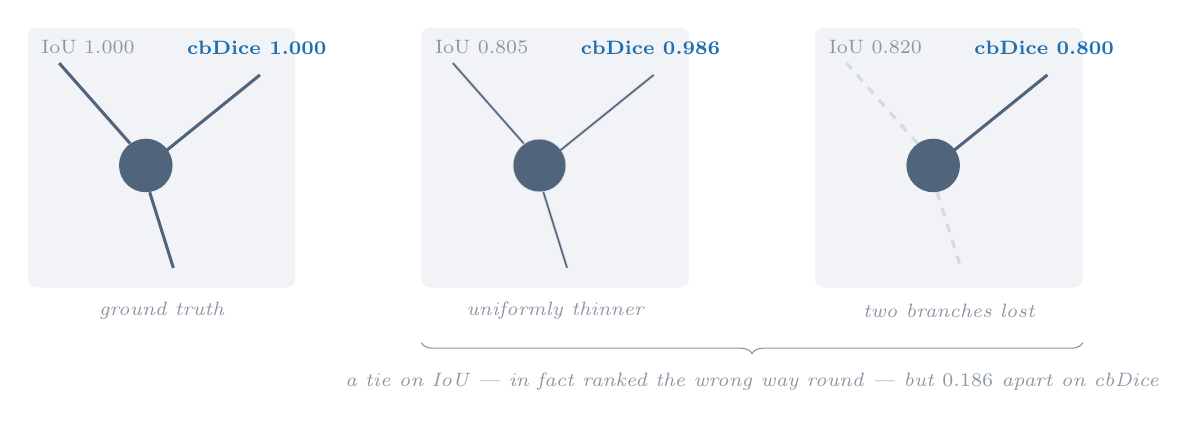
\begin{tikzpicture}[font=\small]
% --- schematic: two errors an area metric cannot tell apart -------------
% Values are MEASURED on exactly the shapes drawn here (soma disc of radius
% 0.34 cm plus three 1.1 pt segments, rasterised at 100 px/cm), by
% benchmark/why_topology.py. Nothing here is illustrative.
%   ground truth        IoU 1.000  cbDice 1.000  clDice 1.000
%   uniformly thinner   IoU 0.805  cbDice 0.986  clDice 0.998
%   two branches lost   IoU 0.820  cbDice 0.800  clDice 0.674
% The eroded panel is drawn with radius 0.33 cm and line width 0.531 pt,
% which IS a one-pixel erosion of the shape at left at this rasterisation.
% NB: do not name a \foreach variable \cap - it clashes with LaTeX's \cap
\foreach \dx/\mode/\iou/\cbd/\subcap in {%
    0/0/1.000/1.000/{ground truth},
    5.0/1/0.805/0.986/{uniformly thinner},
    10.0/2/0.820/0.800/{two branches lost}} {
  \begin{scope}[xshift=\dx cm]
    \fill[softgrey!50, rounded corners=3pt] (-1.5,-1.55) rectangle (1.9,1.75);
    \ifnum\mode=1
      % ghost of the true outline, then the eroded shape on top
      \fill[navy!20] (0,0) circle (0.34);
      \draw[navy!20, line width=1.1pt] (0.25,0.18) -- (1.45,1.15);
      \draw[navy!20, line width=1.1pt] (-0.2,0.28) -- (-1.1,1.3);
      \draw[navy!20, line width=1.1pt] (0.05,-0.34) -- (0.35,-1.3);
      \fill[navy!75] (0,0) circle (0.33);
      \draw[navy!75, line width=0.531pt] (0.25,0.18) -- (1.45,1.15);
      \draw[navy!75, line width=0.531pt] (-0.2,0.28) -- (-1.1,1.3);
      \draw[navy!75, line width=0.531pt] (0.05,-0.34) -- (0.35,-1.3);
    \else
      \fill[navy!75] (0,0) circle (0.34);
      \draw[navy!75, line width=1.1pt] (0.25,0.18) -- (1.45,1.15);
      \ifnum\mode=0
        \draw[navy!75, line width=1.1pt] (-0.2,0.28) -- (-1.1,1.3);
        \draw[navy!75, line width=1.1pt] (0.05,-0.34) -- (0.35,-1.3);
      \else
        % the two deleted branches, as faded ghosts
        \draw[navy!18, line width=1.1pt, dashed] (-0.2,0.28) -- (-1.1,1.3);
        \draw[navy!18, line width=1.1pt, dashed] (0.05,-0.34) -- (0.35,-1.3);
      \fi
    \fi
    \node[font=\scriptsize\itshape, text=midgrey] at (0.2,-1.85) {\subcap};
    \node[font=\scriptsize, anchor=west, text=midgrey] at (-1.45,1.5)
         {IoU \iou};
    \node[font=\scriptsize\bfseries, anchor=west, text=ourblue] at (0.4,1.5)
         {cbDice \cbd};
  \end{scope}}
% brace tying the two error panels together
\draw[decorate, decoration={brace, amplitude=4pt, mirror}, draw=midgrey]
     (3.5,-2.25) -- (11.9,-2.25);
\node[font=\scriptsize\itshape, text=midgrey, align=center]
     at (7.7,-2.75)
     {a tie on IoU --- in fact ranked the wrong way round ---
      but $0.186$ apart on cbDice};
\end{tikzpicture}
\caption{\textbf{Why an area metric is not enough.} Two different failures,
measured on exactly the shapes drawn. The middle mask is topologically
perfect but one pixel too thin everywhere; the right-hand mask keeps its
thickness but has lost two of its three branches. IoU cannot separate them,
and in fact prefers the mask that has lost the branches ($0.820$ against
$0.805$), because at this rasterization the branches are only about four
pixels wide and thinning the whole shape costs more area than deleting them.
cbDice orders the two correctly and by a wide margin ($0.986$ against
$0.800$; clDice $0.998$ against $0.674$). For neurite outgrowth it is the
right-hand failure that destroys the measurement, and it is the one an area
metric is blind to.}
\label{fig:whytopology}
\end{figure}

Frame 0 contains the initial annotations used to prompt both NeuroVestigo and the baseline SAM\,2; hence it is excluded from all quantitative evaluations. Consequently, all methods are assessed exclusively on the subsequent propagated frames ($t \ge 1$) across the four held-out recordings, comprising a total of 328 evaluation frames. Metrics are calculated on a per-frame basis using hard masks at the native resolution of each recording. For methods that require upsampled inputs, predictions are rescaled back to the native resolution prior to evaluation, ensuring a standardized spatial domain for all comparisons. To prevent longer sequences from disproportionately influencing the aggregate results, frame-level metrics are first averaged within each recording, and these recording-level scores are then weighted equally. Table~\ref{tab:main} reports the resulting means and standard deviations across the four test recordings. 

%=====================================================================
\section{Results}
\label{sec:results}

\subsection{Comparison with existing methods}
\label{sec:res:benchmark}

Table~\ref{tab:main} compares NeuroVestigo against six methods,
spanning four distinct algorithmic families, on the four held-out recordings.
Notably, our proposed approach outperforms all methods across every metric.
The evaluated methods differ significantly in both their per-frame input
requirements and output representations. Both NeuroVestigo and the baseline
SAM\,2 are initialized identically with a single ground-truth mask at
frame~0, which is then propagated across the sequence to maintain consistent
object identity temporally. In contrast, $\mu$SAM requires a ground-truth
bounding box prompt on every frame --- representing the highest degree of
per-frame supervision among the compared methods --- yet still yields
inferior performance across all metrics. Finally, the three fully automatic
methods require no prompting but process each frame independently, segmenting
all objects in the field of view without establishing temporal
correspondence. Consequently, isolating a single target and preserving its
identity throughout the recording for these methods necessitates an external
matching heuristic, as detailed below.

\begin{table}[!htb]
\centering
\caption{\textbf{Held-out test-set performance.} Evaluated on four strictly
held-out recordings (excluding the frame-0 prompt), with required per-frame
supervision noted to contextualize the comparisons. Our proposed model
significantly outperforms all methods across both topological metrics by a
substantial margin. Furthermore, these results expose the limitations of
area-based evaluation: $\mu$SAM and Cellpose-SAM sit within $0.012$ IoU of
one another ($0.575$ vs. $0.563$) yet differ by $0.067$ in structural
connectivity ($0.792$ vs. $0.725$ cbDice). SAM\,3.1 is reported in
both of the modes its video interface accepts; it cannot be given a mask
prompt, and its concept mode is not target-aware, so its predictions are
reduced to the target exactly as for the other automatic methods.}
\label{tab:main}
\small
\begin{tabular}{lcccc l}
\toprule
Method & IoU & Dice & \textbf{cbDice} & clDice & Per-frame supervision \\
\midrule
\textbf{NeuroVestigo}            & \textbf{0.763} & \textbf{0.864} & \textbf{0.855} & \textbf{0.946} & 1 annotation (frame 0) \\
SAM\,2 (zero-shot)       & 0.639 & 0.771 & 0.758 & 0.830 & 1 annotation (frame 0) \\
$\mu$SAM (box-prompt)    & 0.575 & 0.721 & 0.792 & 0.843 & GT box, \emph{every} frame \\
SAM\,3.1 (point-prompt)  & 0.471 & 0.595 & 0.602 & 0.592 & 10 GT points, \emph{every} frame \\
Cellpose-SAM             & 0.563 & 0.708 & 0.725 & 0.798 & none (automatic) \\
NeuroQuantify            & 0.446 & 0.594 & 0.602 & 0.680 & none (automatic) \\
Omnipose                 & 0.279 & 0.428 & 0.560 & 0.649 & none (automatic) \\
SAM\,3.1 (text-prompt)   & 0.200 & 0.278 & 0.260 & 0.290 & none (automatic) \\
\midrule
\multicolumn{2}{l}{\emph{our margin over best method}} & & $0.064$ & $0.103$ & \\
\bottomrule
\end{tabular}
\end{table}


The empirical performance of each method closely aligns with its underlying
design priorities (Figure~\ref{fig:benchmark}). The baseline SAM\,2 reliably
segments the main soma but fails to delineate fine, low-contrast processes,
attaining an IoU of $0.639$ and a cbDice of $0.758$. Despite benefiting from
a per-frame bounding box prompt, $\mu$SAM achieves only $0.575$ IoU and
$0.792$ cbDice. Notably, Cellpose-SAM nearly matches $\mu$SAM in regional
overlap ($0.563$ IoU) but underperforms significantly in preserving
topological connectivity ($0.725$ cbDice). This discrepancy perfectly
illustrates the divergence between the two metric families discussed in
Section~\ref{sec:met:metrics}. Finally, the domain-specific methods trail
further behind: NeuroQuantify attains an IoU of $0.446$, while Omnipose
reaches just $0.279$. The latter severely fragments the target into a median
of eighteen distinct instances per frame, necessitating extensive reassembly
by the external matching heuristic.

SAM\,3.1 lacks the direct mask-based initialization utilized by our
architecture and SAM\,2; its temporal interface is strictly restricted
to text, point, and bounding box prompts. Even when provided with dense
supervision of ten ground-truth points per frame, SAM\,3.1 achieves an
IoU of just $0.471$, which further plummets to $0.200$ in its native
text-based prompt mode. Consequently, an architecture an order of
magnitude larger than our selected backbone substantially underperforms
zero-shot SAM\,2, despite requiring significantly heavier per-frame
supervision. On the \texttt{A12\_C1\_100k\_2} recording, the text-based
prompt failed to generate any prediction overlapping the target
(yielding a raw foreground of $0.0004$ and $0.1$ instances per frame),
whereas the point-prompted configuration reached $0.544$ IoU on the
identical sequence. This massive discrepancy confirms that the semantic
language interface is the primary point of failure. Crucially, this
deficit originates in target specification rather than temporal
propagation. Because SAM\,3.1 also integrates robust inter-frame memory,
its underperformance relative to SAM\,2 stems entirely from how the
object is defined, not how it is tracked. A segmentation mask inherently
encapsulates the complete topological complexity of the target.
Conversely, sparse visual priors (points and boxes) or purely semantic
text descriptions cannot capture this structural nuance --- an omission
that is trivial for compact cells but highly detrimental for arborized
geometries like a neuron.

\begin{figure}[!htb]
  \centering
  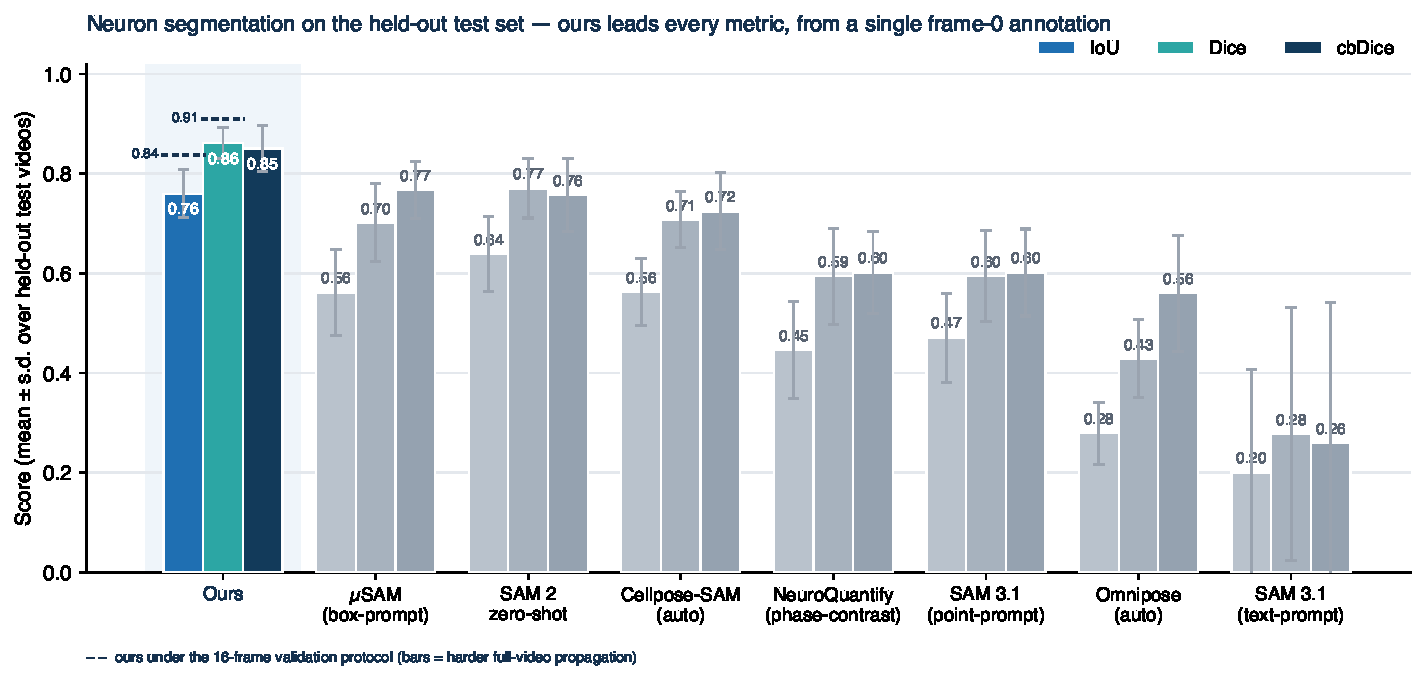
\includegraphics[width=0.92\textwidth,height=0.414\textwidth,keepaspectratio]{fig_benchmark_test}
  \caption{\textbf{Segmentation accuracy on the held-out test set.} Bars give
  IoU, Dice and cbDice, scored on propagated frames ($t\ge1$); competing
  methods are ordered by cbDice. Each recording is averaged over its own
  frames first, so the bar is the mean of four recording-level scores and the
  error bar is their standard deviation.}
  \label{fig:benchmark}
\end{figure}


Our proposed model attains $0.763$ IoU and $0.855$ cbDice. The comparison
against the baseline SAM\,2 is the most strictly controlled evaluation
available, as both models share identical backbones, prompting mechanisms,
and inference procedures, differing solely in the inclusion of the low-rank
adapters detailed in Section~\ref{sec:met:model}. Consequently, this
adaptation yields an absolute improvement of $+0.124$ IoU and $+0.097$
cbDice, achieved by fine-tuning only $13.9\,\%$ of the network parameters. A
margin of this magnitude is highly significant for targets as diminutive and
intricately branched as these; because the object occupies only a minimal
percentage of the frame, a single pixel of boundary error along a neurite
disproportionately degrades the overall score. Furthermore, the
propagation never fails outright: the lowest per-frame IoU NeuroVestigo records
across the 328 evaluated frames is $0.575$, and no frame falls below $0.3$,
which is not true of any competing method
(Figure~\ref{fig:qualitative}).



All competing methods were evaluated according to their respective authors'
recommended protocols. Any hyperparameters that significantly influence the
output were optimized on the validation split and subsequently held constant
across the held-out recordings. For the fully automated methods, which lack
inherent target awareness, the final prediction is defined as the union of
all generated regions that overlap with the target. Comprehensive
hyperparameter configurations and their corresponding search spaces are
detailed in Appendix~\ref{sec:supp:protocol}.







\subsection{Temporal consistency}
\label{sec:res:temporal}

% NB: an earlier draft claimed quality was "maintained" and stayed
% "essentially flat". Neither is true -- ours falls 0.086 in cbDice from the
% second to the fourth quarter. The defensible claim is the comparative one,
% and it is stronger. Do not restore the old wording.
Although object identity is successfully maintained throughout the sequences,
the topological quality of the predicted masks degrades over time. All
evaluated methods exhibit temporal decay as a recording progresses, and the
rate of this degradation distinguishes the methods more sharply than their
overall average accuracy. By partitioning each recording into temporal
quartiles and averaging the cbDice scores within each, we observe that our
model experiences a minimal degradation of just $0.070$ between the first and
final quartiles, compared to drops ranging from $0.126$ to $0.418$ for all
baseline methods (Table~\ref{tab:drift}, Figure~\ref{fig:temporal}). This
stability is critical for downstream biological analysis. Because phenomena
such as neurite elongation and retraction are quantified by computing the
differences between consecutive masks, algorithmic drift risks confounding
true morphological evolution with segmentation artefacts.

\begin{table}[!htb]
\centering
\caption{\textbf{Temporal consistency across quartiles.} Mean cbDice is
evaluated across temporal quartiles ($Q_1$--$Q_4$). All methods degrade
(`Decay' $= Q_4 - Q_1$), but our single-prompt model is $1.8\times$ more
stable than the best baseline. Strikingly, $\mu$SAM degrades $2.8\times$
faster and SAM\,3.1 $6.1\times$ faster despite exhaustive per-frame
supervision, demonstrating that frame-wise prompting does not confer
inherent temporal consistency.}
\label{tab:drift}
\small
\begin{tabular}{lccccc}
\toprule
Method & Q1 & Q2 & Q3 & Q4 & Decay \\
\midrule
\textbf{NeuroVestigo}            & \textbf{0.878} & \textbf{0.890} & \textbf{0.846} & \textbf{0.807} & $\mathbf{-0.070}$ \\
Cellpose-SAM             & 0.764 & 0.785 & 0.712 & 0.637 & $-0.126$ \\
Omnipose                 & 0.609 & 0.617 & 0.556 & 0.458 & $-0.150$ \\
$\mu$SAM (box-prompt)    & 0.860 & 0.859 & 0.780 & 0.669 & $-0.191$ \\
SAM\,2 (zero-shot)       & 0.846 & 0.806 & 0.730 & 0.649 & $-0.197$ \\
NeuroQuantify            & 0.694 & 0.710 & 0.568 & 0.436 & $-0.258$ \\
SAM\,3.1 (point-prompt)  & 0.778 & 0.731 & 0.539 & 0.360 & $-0.418$ \\
\bottomrule
\end{tabular}
\end{table}


A portion of this performance degradation is attributable to the increasing
complexity of the segmentation task. The target neuron undergoes continuous
growth throughout the recording: between the initial and final quartiles, its
centerline lengthens by a factor of $3.3$, while its mean thickness decreases
from $8.7$ to $7.2$ pixels. Consequently, the target structure becomes
simultaneously more spatially extensive and topologically finer. This
morphological evolution also elucidates why performance in the second
quartile ($Q_2$) generally exceeds that of the first ($Q_1$) across most
methods in Table~\ref{tab:drift}. Because cbDice is normalized by the total
centerline length, and $Q_1$ features the shortest centerlines of the
sequence, any absolute pixel error incurs a disproportionately severe penalty
during these early frames.

\begin{figure}[!htb]
  \centering
  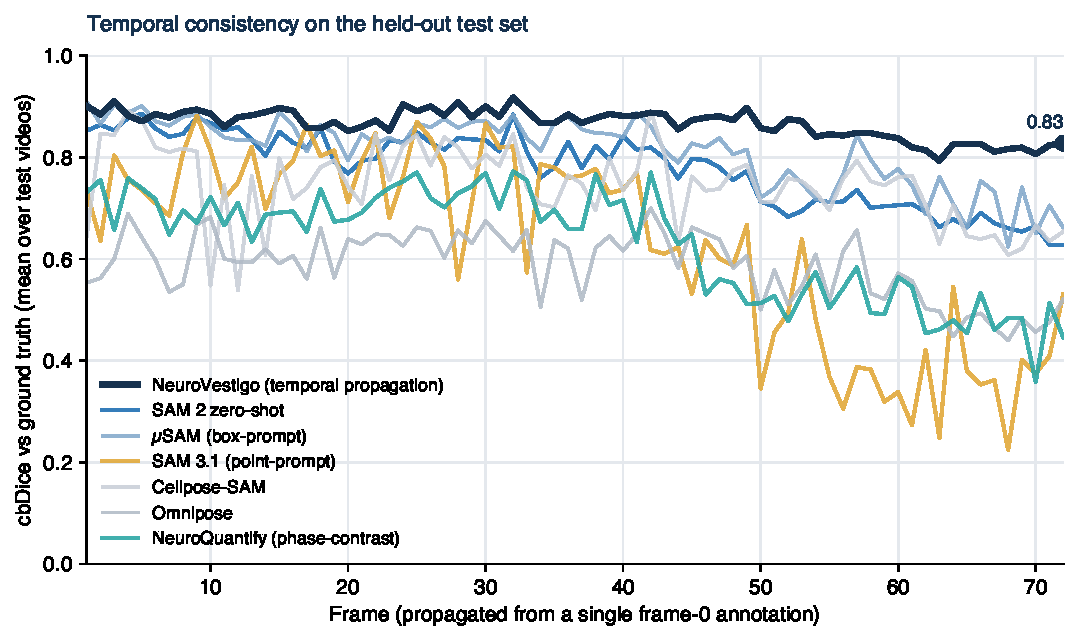
\includegraphics[width=0.92\textwidth,height=0.548\textwidth,keepaspectratio]{fig_temporal_consistency}
  \caption{\textbf{Segmentation quality across the propagated sequence.} Mean
  cbDice at each frame index, averaged over the four held-out recordings,
  with every method prompted or run as described in
  Table~\ref{tab:protocol}. Frame~0 is the given annotation and is excluded.
  NeuroVestigo is prompted once and remains close to its initial quality
  throughout, while the single-frame methods decline steadily; the widening
  separation to the right of the plot is the decay quantified in
  Table~\ref{tab:drift}.}
  \label{fig:temporal}
\end{figure}


That the two methods given ground-truth prompts on \emph{every} frame drift
fastest of all is not the paradox it first appears. A sparse prompt describes a
growing arbor progressively worse: the target fills $29\,\%$ of its own
bounding box in the first quarter of a recording and $14\,\%$ in the last.
Methods that re-derive the object from a box or a handful of points on each
frame therefore work from a description that degrades exactly as the target
becomes harder, whereas a mask-seeded memory carries the full shape forward
from the frames in which it was simplest. Per-frame supervision is not the same
as per-frame information.

Because the memoryless baselines process frames independently, their minimum
decay of $0.126$ strictly isolates the escalating difficulty of the task
itself, independent of accumulated drift. In contrast, our stateful model
restricts this decay to just $0.070$, demonstrating that temporal propagation
actively offsets this rising difficulty by leveraging structural priors from
earlier, simpler frames.





\subsection{Ablations}
\label{sec:res:ablation}

We conducted an ablation study to isolate the impact of three key components.
Each configuration was trained following the schedule detailed in
Section~\ref{sec:met:model} and evaluated using the established protocol.

\emph{Adaptation.} Base SAM\,2 and NeuroVestigo share a backbone, prompt
formulation, and inference procedure, differing exclusively in the learned
adapters. As shown in Table~\ref{tab:main}, this parameter-efficient
adaptation yields an absolute performance gain of $+0.124$ IoU and $+0.097$ cbDice.

\emph{Temporal horizon.} Expanding the training clip length from eight to
sixteen frames doubles the temporal receptive field over which gradients
backpropagate through the memory-attention adapters. This extension actively
mitigates the temporal drift discussed in Section~\ref{sec:res:temporal},
reducing the decay from $0.084$ to $0.070$. Notably, this improvement is
strictly localized to the tail end of the sequence: performance across the
first three quartiles fluctuates by no more than $0.002$, whereas the final
quartile exhibits a $+0.013$ increase. Thus, the extended horizon does not
inherently improve single-frame segmentation fidelity, but rather enhances
long-term target retention. This strongly suggests that the primary
bottleneck for processing lengthy sequences resides within the memory pathway
rather than the mask decoder.

\emph{Training-set size.} We tested directly whether more recordings of the
same kind help. Adding two recordings to the training split --- twenty to
twenty-two, same culture protocol, same modality --- moves the held-out mean
IoU from $0.7599$ to $0.7633$, a difference of $+0.0035$. The direction is
not consistent across recordings: two improve ($+0.0209$, $+0.0076$) and two
degrade ($-0.0080$, $-0.0067$), giving a paired $t = 0.51$ on three degrees
of freedom, $p = 0.65$. Validation moved by a comparable amount, $0.8377$ to
$0.8399$. The temporal decay is unchanged at $0.070$.

The relevant question is not whether this difference is significant --- it
plainly is not --- but what size of effect this benchmark could resolve. The
standard deviation of the paired per-recording difference is $0.0136$, so
with four test recordings a two-sided paired test at $\alpha = 0.05$ requires
$|\Delta\mathrm{IoU}| > 0.0217$. The observed rate is $+0.0017$ IoU per added
recording, so reaching that threshold at this rate would take on the order of
thirteen recordings in total --- roughly eleven beyond the two already
added. We therefore read the model as saturated with respect to recordings of
this kind at this scale: a further recording of the same cell type under the
same protocol contributes samples rather than information, and the benchmark
would not detect its effect even if one existed. This is a weaker claim than
``more data would help'', and a more defensible one; what the evidence
supports is that additional variation --- other culture conditions,
magnifications or cell types --- is the direction likely to matter, not more
of the same.

\emph{Topology weighting.} The two topology terms exhibit markedly
different optimization dynamics. At a coefficient of just $0.3$, the
supervoxel term dominates the training signal, supplying approximately
$75\,\%$ of the weighted gradient norm compared to a mere $4\,\%$ from
the focal term (weighted at $3.0$). Furthermore, its response landscape
is exclusively sensitive to topological integrity. When evaluating
isolated defects, a massive $4096$-pixel volumetric hole in the soma
yields a supervoxel penalty of only $0.016$, whereas a minute
$280$-pixel fracture across a branch spikes the penalty to $1.86$.
Area-based metrics strictly invert this hierarchy: focal and Dice losses
heavily penalize the spatial cavity ($0.0078$ and $0.042$) while
remaining virtually blind to the critical branch split ($0.0005$ and
$0.0057$). Attempting to increase the supervoxel coefficient to $2.0$
degraded validation IoU by $0.017$ while the supervoxel loss itself
plateaued; because smaller increments fell within the margin of
stochastic variance, we retain the $0.3$ weighting. Similarly, scaling
the cbDice coefficient in Eq.~\ref{eq:loss} from $0.3$ to
$1.0$---increasing its contribution from $11\,\%$ to $30\,\%$ of the
total loss---produced no measurable impact. Across the nine combined
validation and test recordings, all paired metric differences remained
strictly bounded by $\pm0.005$, yielding no statistical significance.
Because the loss landscape is insensitive to this hyperparameter within
the operational range, we adopt the smaller weight.

\begin{figure}[!htb]
  \centering
  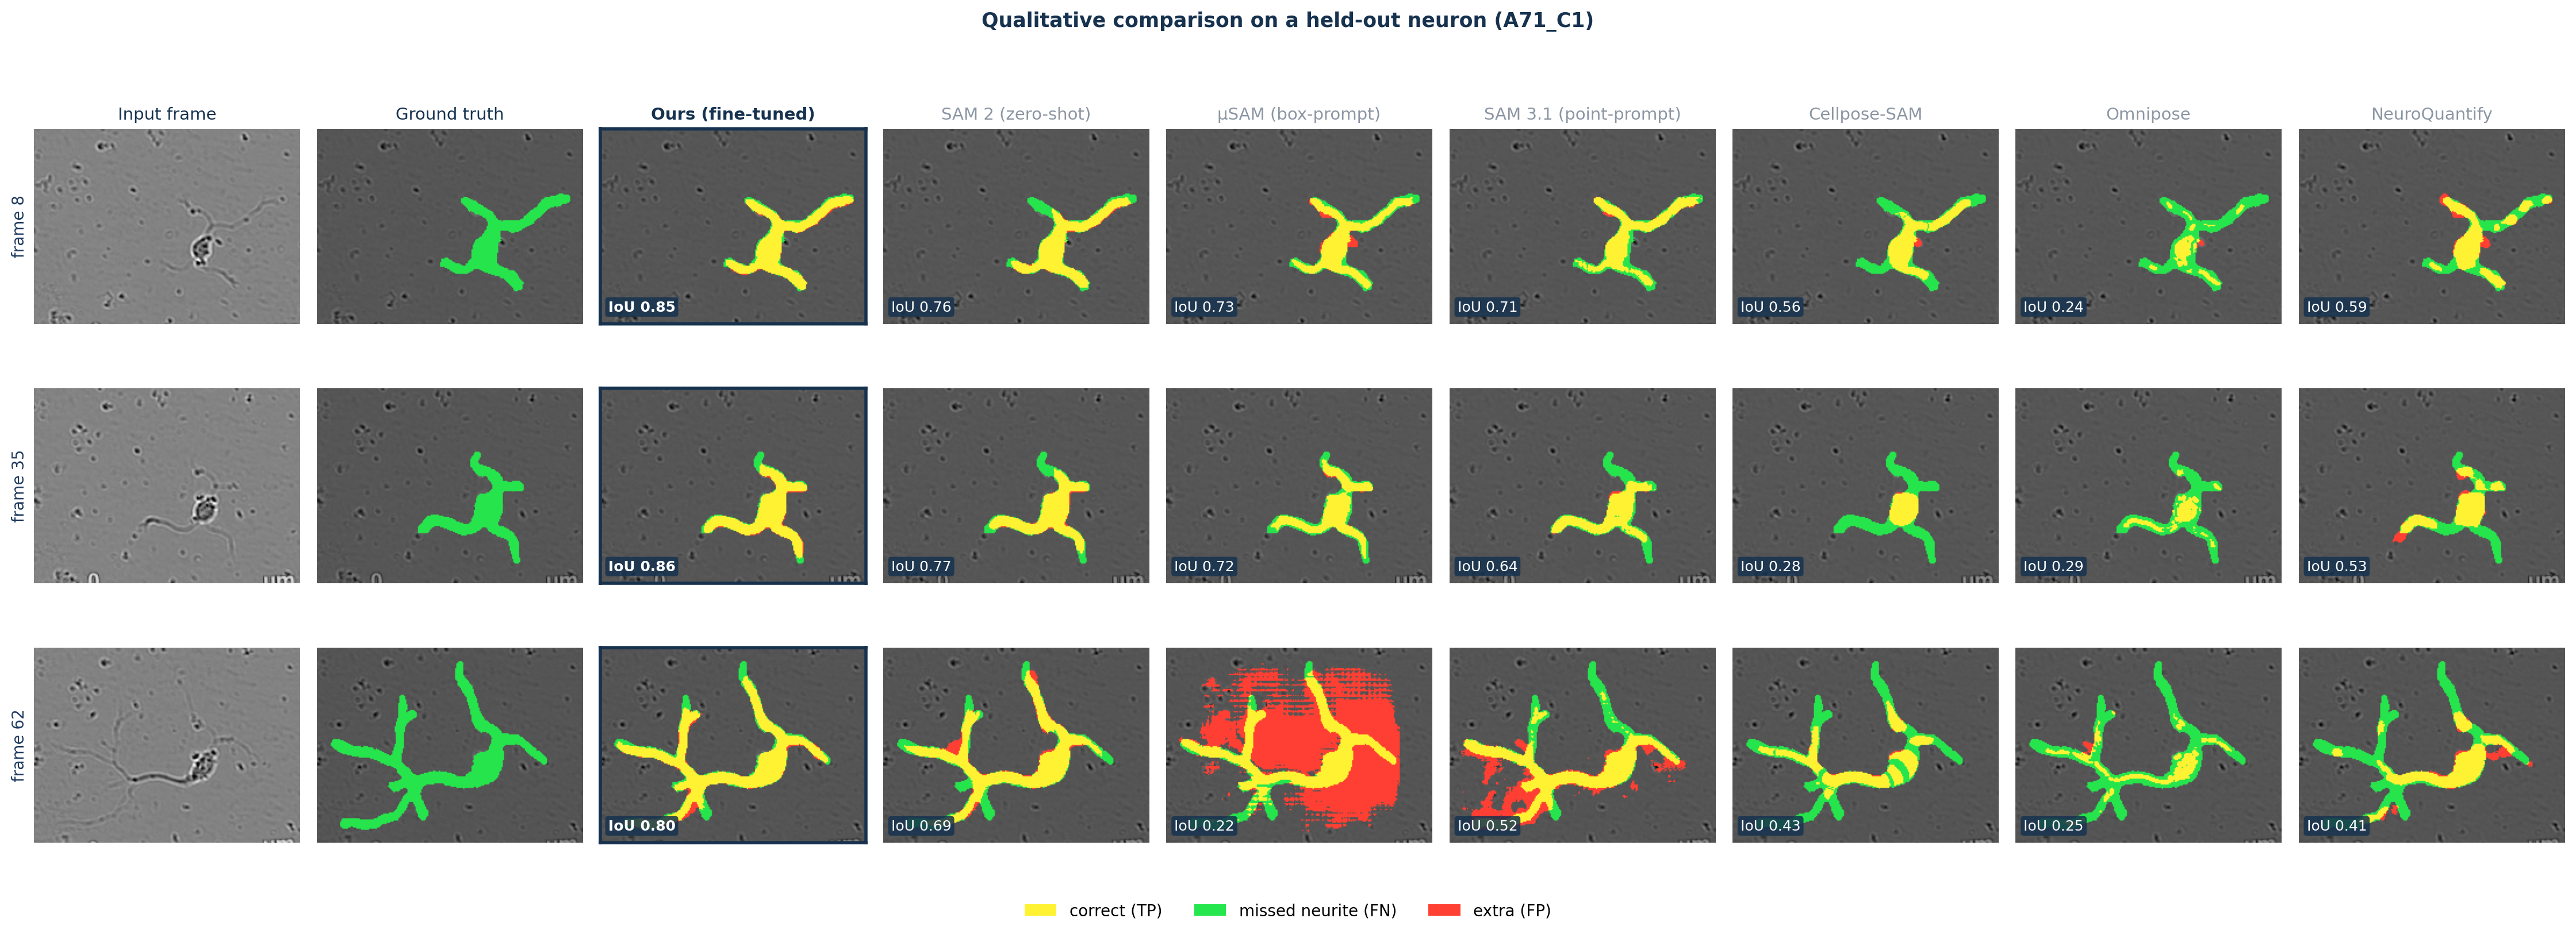
\includegraphics[width=\textwidth,height=0.364\textwidth,keepaspectratio]{proof_A71_C1.png}
  \caption{\textbf{Qualitative comparison on a held-out recording.} Every
  method at three time points of \texttt{A71\_C1}, each run as described in
  Table~\ref{tab:protocol}. Overlay semantics: yellow, correctly segmented;
  green, ground-truth neurite missed; red, predicted pixels outside the
  ground truth; per-panel IoU inset. NeuroVestigo and SAM\,2 are prompted only
  on frame~0 and every subsequent mask is produced by propagation, whereas
  $\mu$SAM and SAM\,3.1 receive ground-truth prompts on the frame shown. The
  progression down the column is the growth that makes the task harder: by
  frame~62 the arbor has roughly tripled in centerline length, and the
  competing methods lose the thin distal branches that NeuroVestigo retains.}
  \label{fig:qualitative}
\end{figure}


%=====================================================================
\section{Discussion}
\label{sec:discussion}

% CAUTION -- claims that are NOT supported, do not restore them:
%  (a) "the margin concentrates on connectivity rather than area". Margin over
%      the best baseline: IoU 0.113, clDice 0.109, Dice 0.086, cbDice 0.080 --
%      the margin is in fact LARGEST on IoU.
%  (b) "cbDice is more sensitive than IoU to losing a branch". Measured on the
%      Fig. whytopology shape at five aspect ratios (branch area 29% down to
%      7%), cbDice tracks IoU to within 0.02 EVERYWHERE. Losing two of three
%      branches costs IoU 0.180 and cbDice 0.200 -- a factor of 1.1, not 3.1.
%      The pre-2026-08-11 values (cbDice 0.71 / 0.44) were computed at the
%      broken topology_resolution=256 and must not be quoted.
%  (c) "IoU ranks Cellpose-SAM above Omnipose, topology metrics reverse it".
%      Dead after the flow_threshold fix: Cellpose-SAM now beats Omnipose on
%      both (IoU 0.563 vs 0.279, cbDice 0.725 vs 0.560).
% Two arguments DO survive, verified by benchmark/why_topology.py, and P1/P2
% are written from them:
%   MATCHED-IoU (Fig. whytopology) -- a 1 px uniform erosion and a two-branch
%     deletion score IoU 0.805 vs 0.820, i.e. IoU ranks them BACKWARDS, while
%     cbDice reads 0.986 vs 0.800 (clDice 0.998 vs 0.674).
%   DISCRIMINATION (Tab. main) -- uSAM and Cellpose-SAM sit within 0.001 on
%     IoU (0.562 / 0.563) yet 0.043 apart on cbDice (0.767 / 0.725).
We introduced a parameter-efficient adaptation of SAM\,2 (via dual-rank
LoRA+) for the longitudinal tracking of highly arborized neurons.
Conditioned on a single initial mask, NeuroVestigo establishes
state-of-the-art performance across all metrics on strictly held-out test
sequences (Table~\ref{tab:main}). Ablations confirm these gains ($+0.124$
IoU, $+0.097$ cbDice) stem entirely from the learned adapters, utilizing
only $13.9\,\%$ of the parameter space. Crucially, our temporal memory
mechanism restricts longitudinal degradation to a mere $0.070$ cbDice,
substantially outperforming memoryless baselines whose decay strictly
reflects the escalating morphological complexity of the target
(Table~\ref{tab:drift}). Competing baselines fundamentally struggle on this
task because their underlying representations lack simultaneous constraints
for topology, temporal identity, and domain-specific appearance. Notably, this single
annotation outperforms $\mu$SAM supplied with a ground-truth bounding box on
\emph{every} frame, the heaviest per-frame supervision in the comparison.

Our analysis further highlights a critical dichotomy between spatial and
topological optimization. Area-overlap metrics (e.g., IoU) paradoxically
penalize minor boundary shifts more severely than catastrophic structural
disconnections (Figure~\ref{fig:whytopology}). Consequently, methods
within $0.012$ IoU of one another (e.g., $\mu$SAM and Cellpose-SAM) diverge
significantly under topological evaluation (a $0.067$ cbDice gap).
Within our training objective, connectivity constraints --- particularly the
supervoxel term --- dictate the primary optimization dynamics. Despite a
deliberately small nominal coefficient of $0.3$, the supervoxel loss
normalizes each error partition by its constituent pixel count. This
amplifies the gradient magnitude of topologically critical pixels by a
factor of $10^{6}$, allowing the term to supply approximately $75\,\%$ of the
total weighted gradient norm at convergence. By doing so, it selectively
penalizes structural fractures (such as broken branches) that the focal and
Dice losses barely register. Interestingly, varying the cbDice loss weight
yielded negligible performance shifts. We hypothesize this inertness occurs
because the differentiable skeletonization is computed on a downsampled
grid, diluting the topological gradient with resampling artefacts.
Nonetheless, evaluations using the strictly unoptimized clDice metric
confirm our topological advantages reflect genuine structural preservation
rather than loss-level overfitting. We therefore recommend that work on
filamentous or branched cells report a connectivity metric alongside IoU
rather than in place of it.

Two additions to training follow from this and are described in
Section~\ref{sec:met:loss}; neither is yet evaluated on the test set. The
first distils the prompt pathway into the memory pathway: the same weights,
decoding the same frame with its ground-truth mask supplied as a dense
prompt, reach a quality the memory pathway does not, and that output
supervises the memory pathway directly. This is the privileged-information
setting of \cite{lopezpaz2016unifying} rather than generic self-distillation
--- one network, one set of weights, differing only in access to information
withheld at inference. The second withholds the frame-0 prompt during
training, removing a conditioning regime the model was trained in but is never
evaluated in \cite{bengio2015scheduled}.

The analysis around Eq.~\ref{eq:displacement} is worth separating from
whether this particular model improves. An auxiliary distillation loss whose
teacher holds privileged information cannot reach zero, because the student
is denied the information the target was produced with. Its gradient
therefore never vanishes, and the trained model settles not at the optimum of
the supervised objective but at a point displaced from it in proportion to the
weight on that loss. The consequence is practical: such a term is a
regulariser with a bias attached, and the weight is the dial between them, not
a detail to be tuned by search. Our first configuration set it high enough
that the bias dominated, and the resulting model converged early and below
baseline --- which is the predicted behaviour, not an anomaly. We state this
because the same reasoning applies to any auxiliary objective built on a
teacher that the student structurally cannot match, a construction that is
becoming common.
\todo{No test-set results yet. If the current configuration does not beat the
baseline either, the contribution here is the conditioning-gap measurement and
the displacement analysis, not the method --- report it that way and do not
dress it as a win. Update this paragraph, the Results section and
Table~\ref{tab:main} once the run has been benchmarked.}

We acknowledge several limitations. First, our evaluation is constrained to
a small held-out test set (four recordings); thus, our conclusions rely on
consistent metric trends rather than absolute margins. Second, the current
evaluation avoids dense multi-neuron fields with intersecting processes,
representing a likely failure mode in practice. Third, our framework
necessitates a full mask for the initial prompt. While bounding boxes offer
a lower annotation burden, our empirical data indicates that a branched
target fills only $21\,\%$ of its own bounding box on average, falling from
$29\,\%$ in the first quarter of a recording to $14\,\%$ in the last,
suggesting that a box provides a highly ambiguous spatial prior. Finally,
baseline comparisons rely on input scales optimized strictly on the
validation split.

To facilitate future research, we release our annotated sequences as a novel
public benchmark for single-target, temporally propagated neurite
segmentation. Future work will extend this framework to dense, multi-neuron
environments by integrating collision-resolution protocols. Ultimately, once
the derived quantities are validated against manual tracing
\cite{berkovich2025neurite}, the high spatiotemporal consistency achieved by
NeuroVestigo enables the automated, high-throughput extraction of longitudinal
biological metrics --- such as neurite elongation and branching rates ---
directly from sequential masks.

%=====================================================================
\section*{Data and code availability}

All data, code and model weights required to reproduce this work are
publicly available.

\emph{Dataset.} The thirty-two annotated phase-contrast recordings and masks are deposited at Zenodo, \todo{Zenodo DOI}.

\emph{Training and evaluation code.} Adaptation, training and the full benchmark are at
\url{https://github.com/adioiz/NeuroVestigo}.

\emph{Model and plug-in.} The weights and the \texttt{neurons-labeling} napari plug-in are at
\url{https://github.com/adioiz/neurons-labeling}.

\section*{Acknowledgements}
\todo{Funding: agency names and grant numbers, to be supplied by O.S.}
Training and evaluation were carried out on the GPU cluster of the Faculty
of Engineering, Bar-Ilan University. The time-lapse dataset was acquired and
hand-annotated by E.\,N.~Berkovich as part of the M.Sc.\ research reported in
\cite{berkovich2025neurite}. We thank the members of the Shefi laboratory for
preparing the primary cultures and for maintaining the live-imaging system on
which these recordings were made.

During the preparation of this manuscript the authors used Claude (Anthropic)
to draft and edit text and to generate figure and analysis code. All output
was reviewed and verified by the authors, who take full responsibility for
the content of the published article.

\section*{Author contributions}
\begin{sloppypar}
Contributions are stated using the CRediT taxonomy. Adi Oizerovich:
conceptualization, methodology, software, formal analysis, validation,
visualization, writing --- original draft. Efrat Naomi Berkovich:
investigation, data curation, resources, writing --- review and editing.
Sharon Cohen: writing --- review and editing. Ofek Ophir: writing --- review
and editing. Orit Shefi: supervision, project administration, funding
acquisition, resources, writing --- review and editing. All authors read and
approved the final manuscript.
\end{sloppypar}

\section*{Declaration of interests}
The authors declare no competing interests.

%=====================================================================
\appendix
\section{Supplementary figures}
\label{sec:appendix}

\subsection*{How the competing methods were run}
\label{sec:supp:protocol}

\begin{sloppypar}
Two settings recur across the competing methods. The first is input scale:
our recordings are about $1.5$ px per micrometer, coarser than the
magnifications these models were trained at. The second is detection
sensitivity, where library defaults are calibrated for compact,
well-contrasted cells rather than for processes one or two pixels wide.
$\mu$SAM uses the \texttt{vit\_l\_lm} backbone (\texttt{vit\_b\_lm} scores
$0.42$ against $0.56$ validation IoU); Cellpose-SAM uses
\texttt{cellprob\_threshold}~$=-1.0$ ($0.38$ against $0.47$) with
\texttt{flow\_threshold}~$=1.5$ ($0.44$ against $0.56$); Omnipose uses
\texttt{bact\_phase\_omni}, the only one of its models that detects anything
here. Every value was selected on validation and applied unchanged to test;
Table~\ref{tab:protocol} sets out the full configuration.
\end{sloppypar}

$\mu$SAM's mask selection was audited. SAM returns three candidate masks for
an \emph{ambiguous} prompt --- subpart, part and whole of the same object ---
and a single mask otherwise; its documentation reserves the three-mask mode
for sparse prompts such as a lone click and recommends
\texttt{multimask\_output=False} for a box, which is unambiguous. We
therefore report $\mu$SAM in single-mask mode. Keeping $\mu$SAM's own
highest-scoring candidate of three scores marginally higher on validation
($0.595$ against $0.574$ IoU) but lower on the test recordings ($0.562$
against $0.575$ IoU, $0.767$ against $0.792$ cbDice), and it produces the
box-filling selections audited in
\texttt{benchmark/sweep\_usam\_multimask.py}: on $9\,\%$ of test frames,
none earlier than $71\,\%$ through a recording, $\mu$SAM's confidence ranks
a mask more than three times the ground-truth area above a better one it
produced at the same time. Both configurations are scored in the repository
(\texttt{usam} and \texttt{usam\_multimask}); the single-mask mode is used
throughout the paper.

Figure~\ref{fig:proofA81} repeats the qualitative comparison of
Figure~\ref{fig:qualitative} on a second held-out recording, and
Figure~\ref{fig:rawoutput} shows each method's native output before
reduction to the target.

One asymmetry runs against our own model: its object-presence head receives
no supervision under Eq.~\ref{eq:loss} and is disabled at inference, whereas
stock SAM\,2 retains its pretrained head and can decline to segment a frame
it judges empty.

\begin{table}[!htb]
\centering
\caption{\textbf{How each method was run.} Methods differ in how much
information they receive per frame. NeuroVestigo and base SAM\,2 receive a
single annotation for the whole recording; $\mu$SAM receives the
ground-truth bounding box on \emph{every} frame. Input scale, backbone and
detection thresholds were all chosen on the validation split only and applied
unchanged to the test recordings: $\mu$SAM uses the \texttt{vit\_l\_lm}
backbone (\texttt{vit\_b\_lm} scores $0.42$ against $0.56$ validation IoU),
Cellpose-SAM uses \texttt{cellprob\_threshold}~$=-1.0$ (its default of $0$
discards the faintest neurites, $0.38$ against $0.47$) together with
\texttt{flow\_threshold}~$=1.5$ (its default of $0.4$ rejects the target
outright on a large fraction of frames, $0.44$ against $0.56$), and Omnipose
uses
\texttt{bact\_phase\_omni}, the only one of its models that detects anything
here --- \texttt{cyto2\_omni} returns no objects on any validation frame.}
\label{tab:protocol}
\small
\begin{tabular}{l L{2.9cm} L{2.8cm} c L{3.2cm}}
\toprule
Method & Mode used & Prompt per frame & Scale & Reduction to target \\
\midrule
\textbf{NeuroVestigo}      & promptable video propagation & frame 0 only        & $\times$1 & --- single object \\
SAM\,2             & promptable video propagation & frame 0 only        & $\times$1 & --- single object \\
$\mu$SAM           & interactive box prompt       & GT box, every frame & $\times$1 & --- box selects target \\
SAM\,3.1           & promptable video tracking    & 10 GT points, every frame & $\times$1 & --- points select target \\
SAM\,3.1 (text)    & promptable concept segmentation & \texttt{cells}, cap 64 & $\times$1 & union of overlapping instances \\
NeuroQuantify      & automatic, semantic          & none                & $\times$4 & union of overlapping regions \\
Omnipose           & automatic, instance          & none                & $\times$3 & union of overlapping instances \\
Cellpose-SAM       & automatic, instance          & none                & $\times$2 & union of overlapping instances \\
\bottomrule
\end{tabular}
\end{table}

\begin{figure}[!htb]
  \centering
  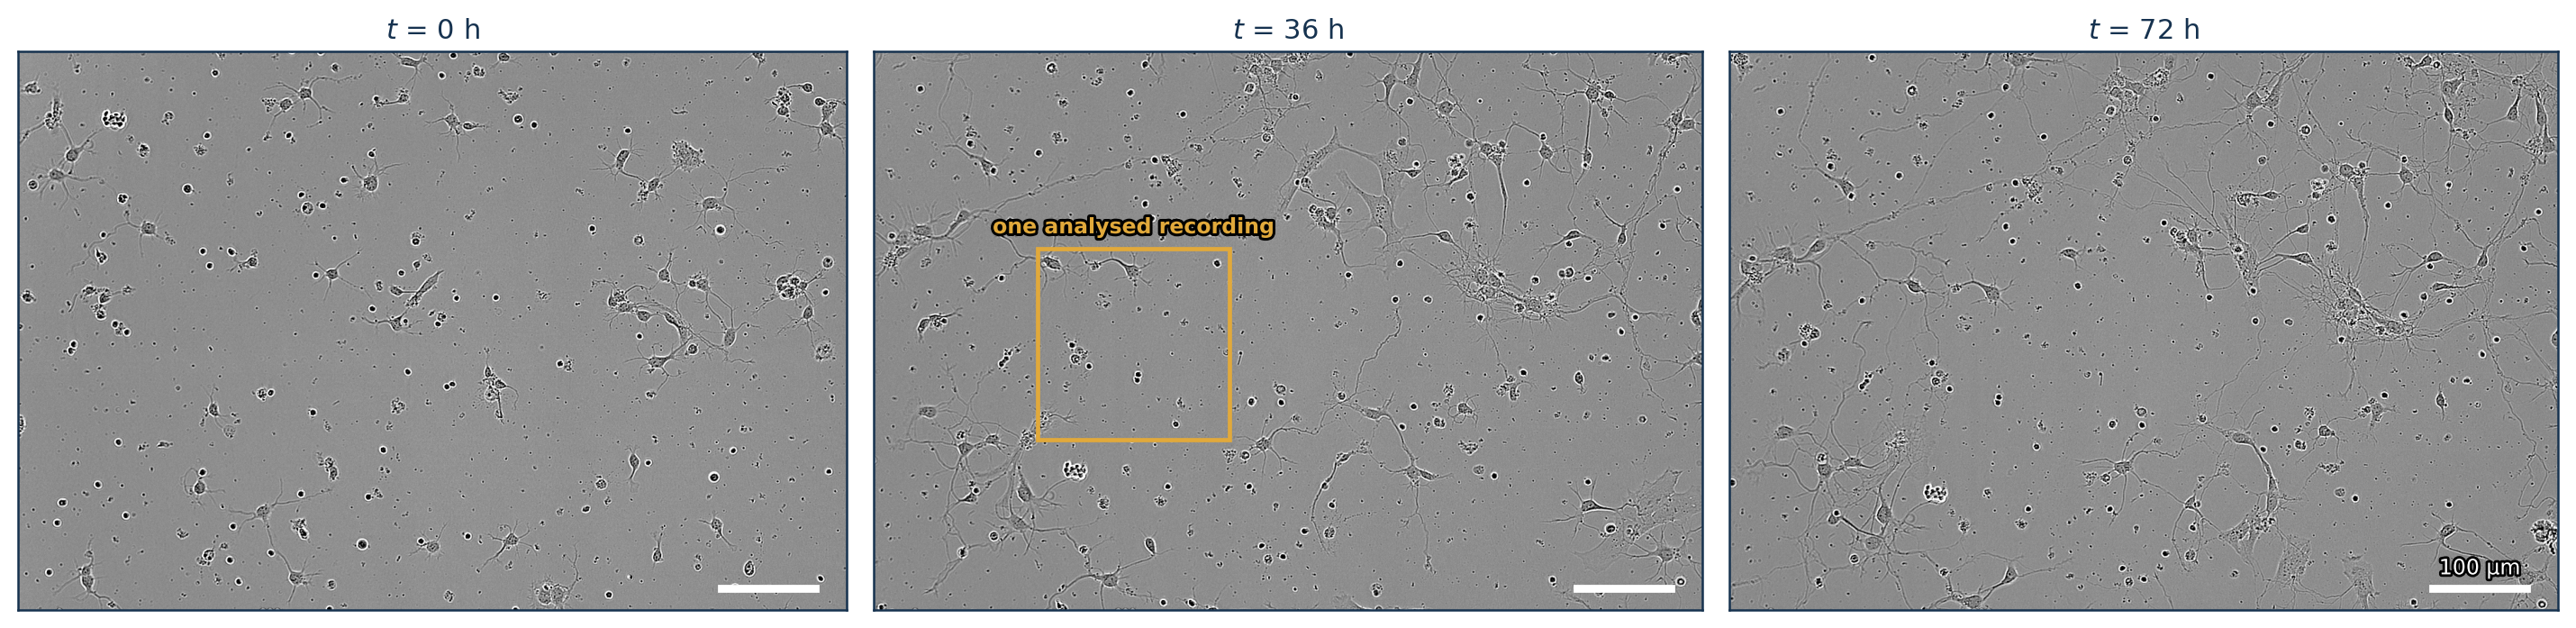
\includegraphics[width=\textwidth,height=0.244\textwidth,keepaspectratio]{figS_culture_field.png}
  \caption{\textbf{Primary cortical culture imaged label-free over 93\,h.}
  A single full IncuCyte field ($843\times568\,\mu$m, $1264\times852$
  pixels) at three time points, showing progressive neurite outgrowth and
  network formation from a sparse plating. Contrast is stretched identically
  across panels for display only. The amber box marks the footprint of one
  analyzed recording ($292\times292$ pixels, $195\times195\,\mu$m): every
  recording used in this work is such a crop, centered on a single target
  neuron. Neighboring cells and debris of similar appearance are present
  throughout, which is why segmenting \emph{a specified} neuron rather than
  all cells is the task.}
  \label{fig:culture}
\end{figure}

\begin{figure}[!htb]
  \centering
  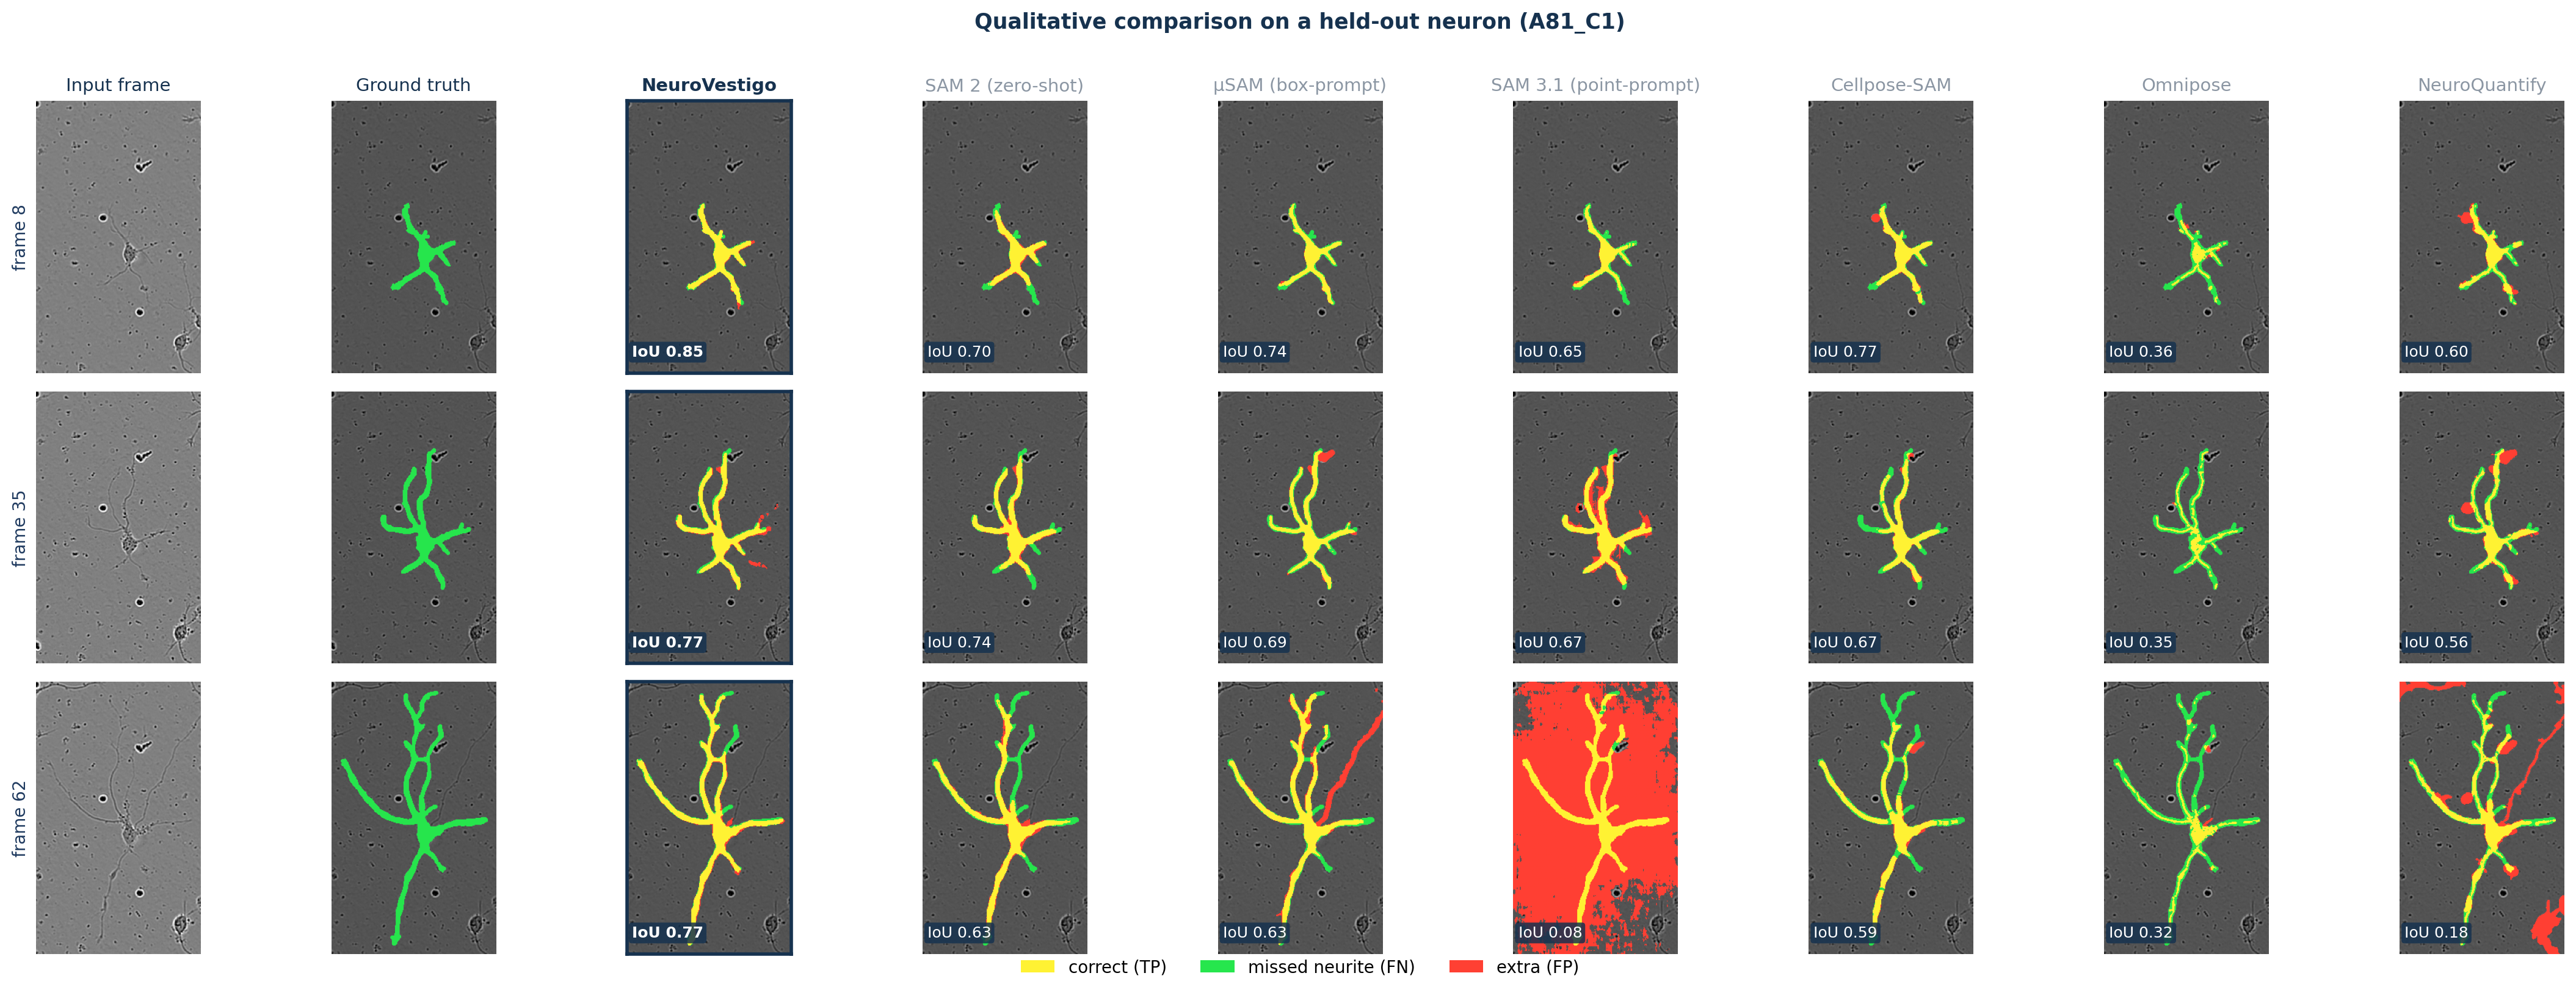
\includegraphics[width=\textwidth,height=0.386\textwidth,keepaspectratio]{proof_A81_C1.png}
  \caption{\textbf{Qualitative comparison on a second held-out recording.}
  As Figure~\ref{fig:qualitative}, for \texttt{A81\_C1}. Overlay semantics:
  yellow, correctly segmented; green, ground-truth neurite missed; red,
  predicted pixels outside the ground truth; per-panel IoU inset.}
  \label{fig:proofA81}
\end{figure}

\begin{figure}[!htb]
  \centering
  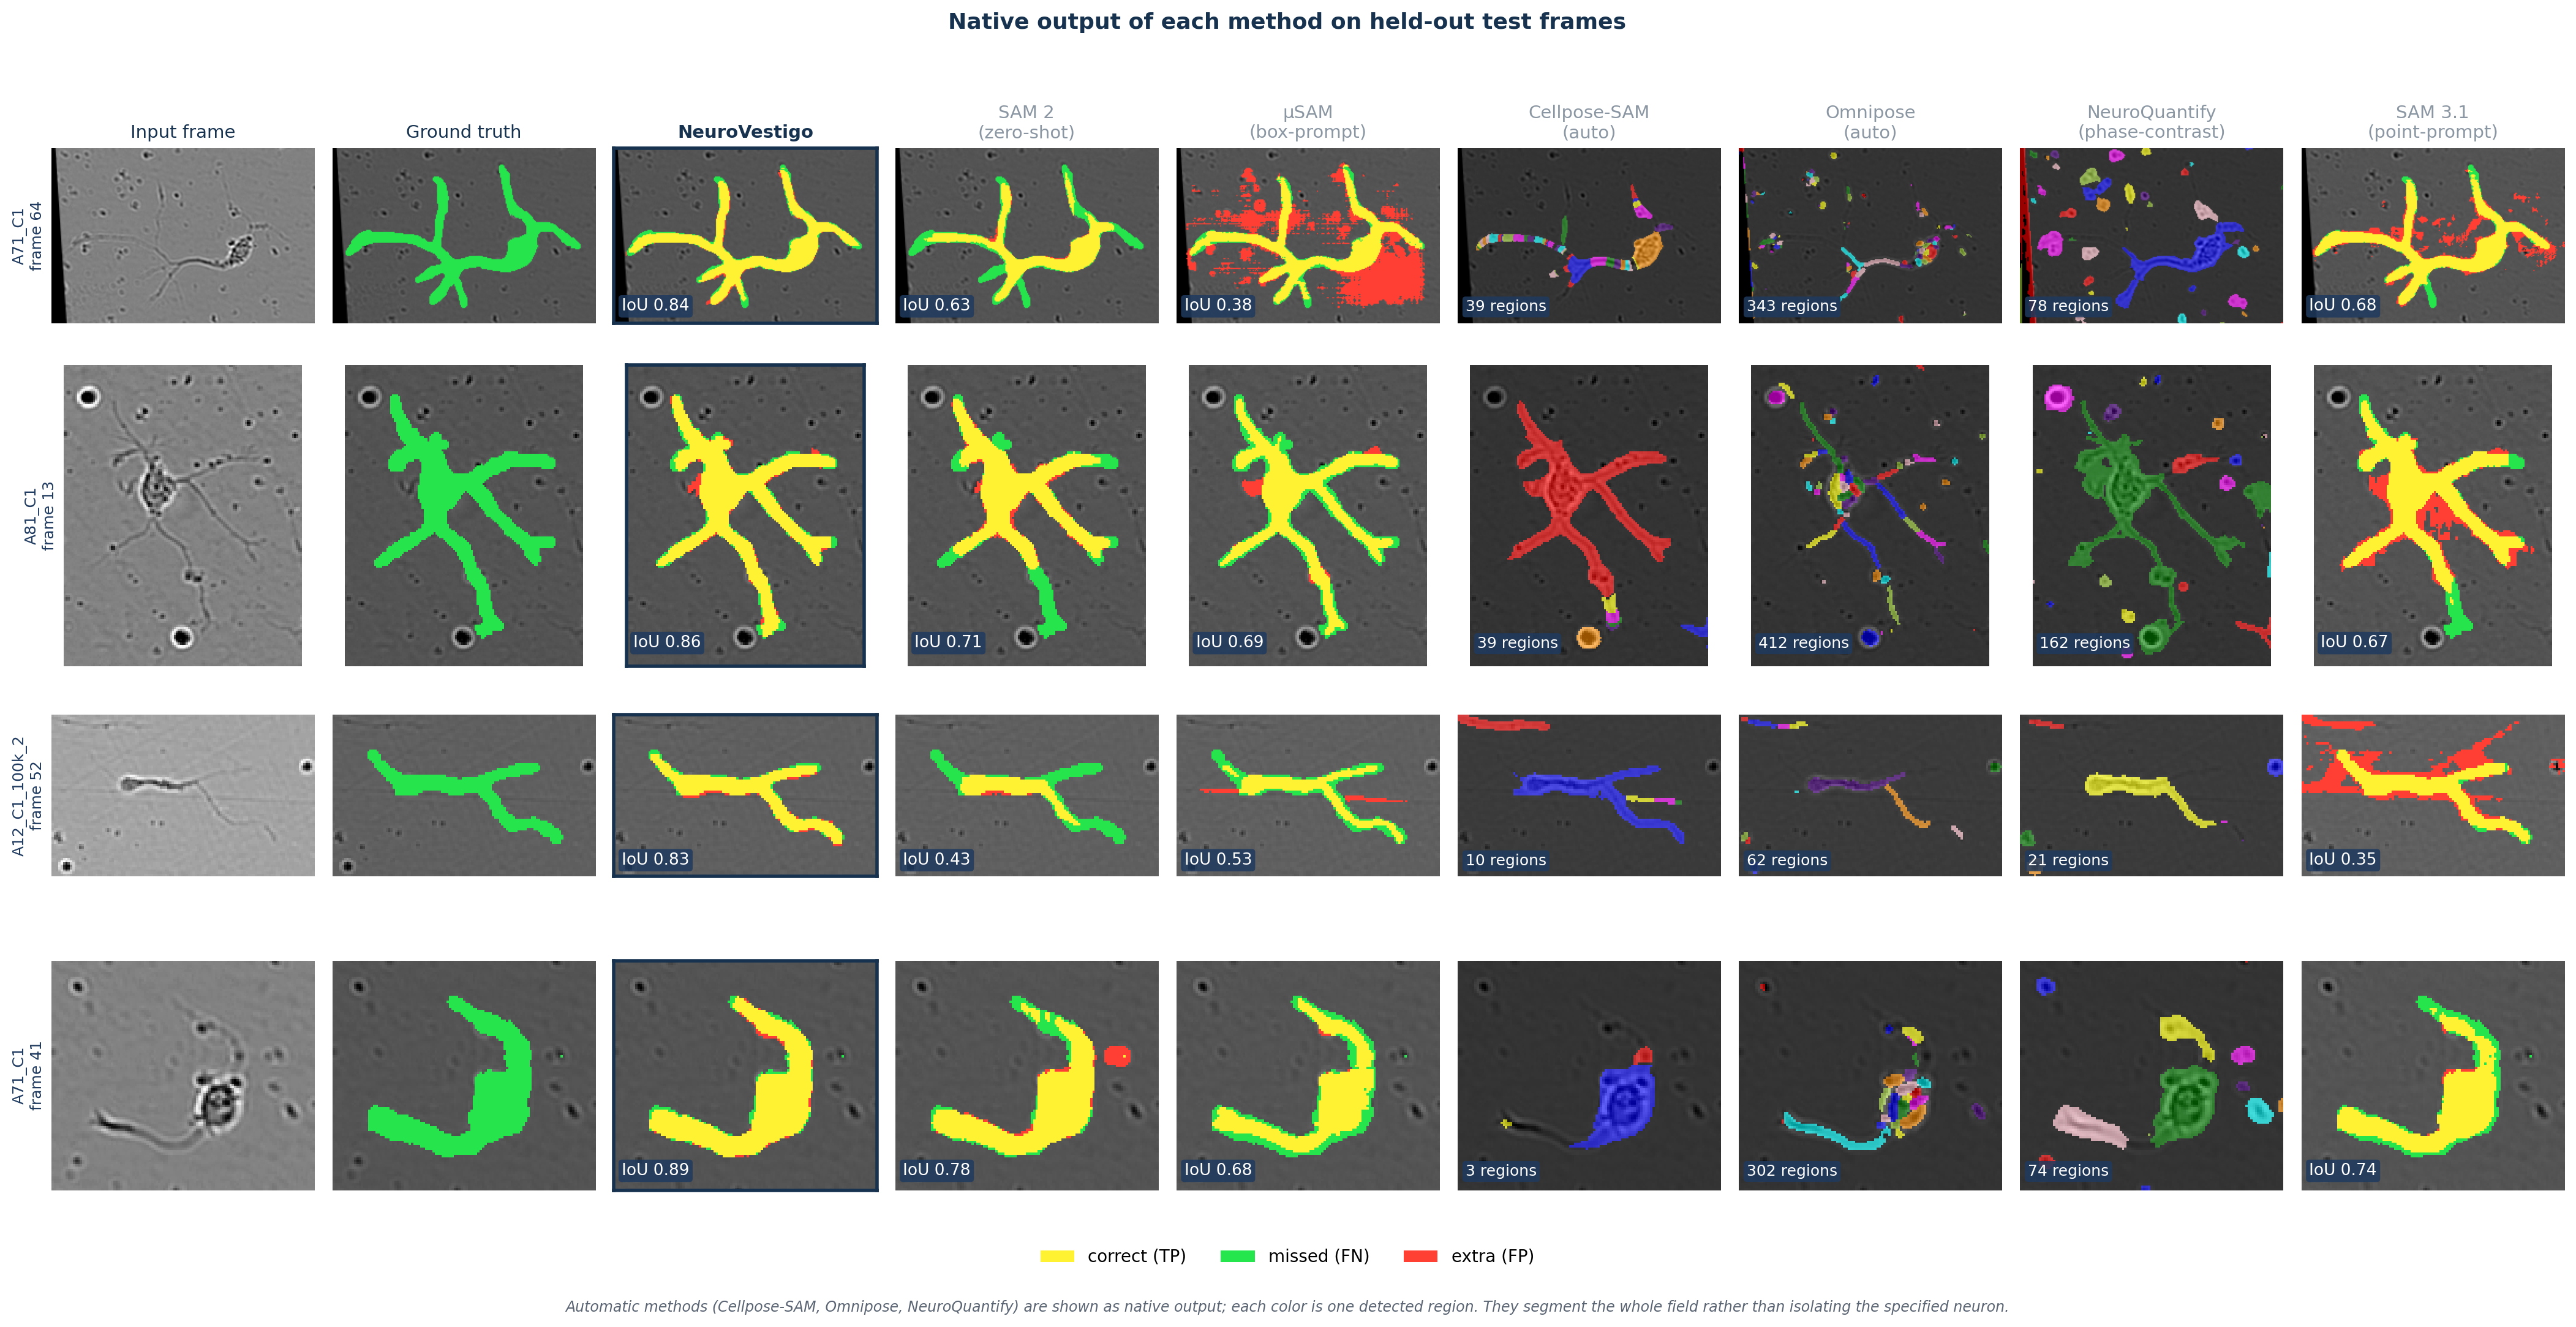
\includegraphics[width=\textwidth,height=0.515\textwidth,keepaspectratio]{single_frame_compare_test.png}
  \caption{\textbf{Raw output of each method, run as designed.}
  The automatic methods are shown as their native
  multi-instance output --- each color is one detected region --- rather
  than after reduction to the target, making explicit that they segment the
  field rather than isolating a specified neuron. NeuroVestigo and the
  promptable baselines are shown as target overlays with per-frame IoU.}
  \label{fig:rawoutput}
\end{figure}

%---------------------------------------------------------------------
% Remove \nocite{*} once the text cites properly - with unsrtnat the
% reference numbers then follow the order of first citation automatically.
\nocite{*}
\bibliographystyle{unsrtnat}
\bibliography{refs}

\end{document}
